% Created 2017-10-05 Thu 16:11
% Intended LaTeX compiler: pdflatex
\documentclass[manuscript=suppinfo,email=true,hyperref=true,keywords=false]{achemso}
\usepackage{times}
\usepackage{float}
\usepackage{amsmath}
\usepackage{amssymb}
\usepackage{graphicx}
\usepackage{hyperref}
\usepackage[T1]{fontenc}
\usepackage{ltablex}
\usepackage{footnote}
\usepackage{braket}
\usepackage[colorinlistoftodos,prependcaption,textsize=small]{todonotes}


\usepackage{xr-hyper} 
%\usepackage{xr}
\externaldocument[main-]{paper}

\SectionNumbersOn{}
\renewcommand{\thesection}{S\arabic{section}}
\renewcommand{\theequation}{S\arabic{equation}}



\author{Tian Tian}
\affiliation{Institute for Chemical and Bioengineering, ETH Z{\"{u}}rich,  Vladimir Prelog Weg 1, CH-8093 Z{\"{u}}rich, Switzerland}
\altaffiliation{T. T. and D. S. contributed equally to this work}
\author{Declan Scullion}
\affiliation{School of Mathematics and Physics, Queen's University Belfast, BT7 1NN, United Kingdom}
\altaffiliation{T. T. and D. S. contributed equally to this work}
\author{Dale Hughes}
\affiliation{School of Mathematics and Physics, Queen's University Belfast, BT7 1NN, United Kingdom}
\author{Lu Hua Li}
\affiliation{Institute for Frontier Materials, Deakin University, Waurn Ponds, Victoria, Australia}
\author{Chih-Jen Shih}
\affiliation{Institute for Chemical and Bioengineering, ETH Z{\"{u}}rich,  Vladimir Prelog Weg 1, CH-8093 Z{\"{u}}rich, Switzerland}
\author{Jonathan Coleman}
\affiliation{School of Physics, Centre for Research on Adaptive Nanostructures and Nanodevices (CRANN) and Advanced Materials and BioEngineering Research (AMBER), Trinity College Dublin, Dublin 2, Ireland.}
\author{Manish Chhowalla}
% \affiliation{Materials Science and Engineering, Rutgers University, 607 Taylor Road, Piscataway, New Jersey 08854, USA.}
\affiliation{Department of Materials Science \& Metallurgy, University of Cambridge, CB3 0FS, United Kingdom}
\author{Elton J. G. Santos}
\email{e.santos@qub.ac.uk}
\affiliation{School of Mathematics and Physics, Queen's University Belfast, BT7 1NN, United Kingdom}

\date{}

\title{Electric polarizability as the fundamental variable in the dielectric properties of two-dimensional materials}
%\title{The Unified Nature of the Dielectric Properties of Two-Dimensional Materials}
\begin{document}

\newpage{}



\section*{Table of Contents}

\begin{itemize}
\item Supplementary Section \ref{sec:polarizability-analysis}: Further analysis on the dielectric properties of 2D materials
  
\item Supplementary Section \ref{sec:2D-3D-rescale}: Hypothetical 2D ``dielectric constant'' rescaled from the 3D dielectric constant

  
\item Supplementary Section \ref{sec:theory-1}: Polarizability-based theoretical model

  
\item Supplementary Section \ref{sec:pol-2D-Eg}: Dependence of $\alpha_{\mathrm{2D}}$ on bandgap

  
\item Supplementary Section \ref{sec:gpaw}: Validation of results using a larger 2D material database

\item Supplementary Section \ref{sec:2D-3D}: More discussion about the
  relation between 2D and 3D properties

  \item Supplementary Section \ref{sec:aniso}: More discussions about the dielectric anisotropy
  
\item Supplementary Section \ref{sec:raw}: Raw data from first
  principles calculations

  
\end{itemize}



\pagebreak{}

\section{Further analysis on the dielectric properties of 2D materials}
\label{sec:polarizability-analysis}

In this section we provide more analysis on the dielectric properties
of 2D materials calculated using many-body Green function method 
(G$_0$W$_0$), including electron-hole interactions at the level of the 
Bethe-Salpeter equation (G$_0$W$_0$--BSE), and at the frequency-dependent regime.  


\subsection{Profile of induced dipoles of 2D material}
\label{sec:dipole-plot}
Here we show in detail the
$\Delta {\rho}=\rho(\boldsymbol{E}) - \rho(\boldsymbol{E}=0)$ profile of
the 2H-MoS$_{2}$ slab in main text Figure \ref{main-fig-1}. The
density $\Delta \rho$ is calculated via $\Delta \rho(z) = \frac{1}{S} \int_{S} \Delta \rho (x,y;z) dx dy $, 
where $S$ is the surface of the unit cell perpendicular to the given direction, in this case $z$. 
%
As can be seen in Figure \ref{fig:rho-profile} the induced charges on the
MoS$_{2}$ layer only extends to a width of $\sim{}$12 \AA{} centered at the middle of the layer. This corresponds to about 6 \AA ~from each side. 
When the
SL size $L \gg$12 \AA{} as in the first principle calculations done in
the main text, the induced dipoles from the periodic images do not
interact, and thus give the converged values of $\alpha_{\mathrm{2D}}$.

\begin{figure}[htbp]
 \centering
 \includegraphics[width=0.5\linewidth]{img/SI-dipole-MoS2.pdf}
 \caption{$\Delta \rho$ as a function of $z$ around the
   MoS$_{2}$ layer, corresponding to main text Figure
   \ref{main-fig-1}\textbf{a}. Green and red parts corresponding to negative and
   positive induced charges. The external electric field
   $E_{\mathrm{ext}}$ is 0.01 eV/\AA{}.}
 \label{fig:rho-profile}
\end{figure}

\subsection{Dielectric properties calculated using many-body Green function method and frequency dependency}
\label{ssec:gw}

Here we will show the results of dielectric properties calculated
using many-body Green function method (G$_0$W$_{0}$)
and with electron-hole interactions at the level of the Bethe-Salpeter 
equation (G$_0$W$_{0}$--BSE). We first compare the case of a
monolayer of BN within a varying superlattice $L$ 
calculated using PBE and G$_{0}$W$_{0}$ as shown in Figure \ref{fig:GW-PBE-alpha}. 
%
%
Both $\varepsilon_{\mathrm{SL}}^{\parallel}$ and
$\varepsilon_{\mathrm{SL}}^{\perp}$ do not converge as a function of $L$ 
despite of the separation utilized in the simulations (Figure \ref{fig:GW-PBE-alpha}{\bf a}-{\bf c}). However, corresponding 2D polarizabilities are almost $L$-independent (Figure \ref{fig:GW-PBE-alpha}{\bf b}-{\bf d}). It is worth noting
that since the G$_{0}$W$_{0}$ method has better estimation of the bandgap, $\varepsilon_{\mathrm{SL}}$ and $\alpha_{\mathrm{2D}}$ are smaller using G$_{0}$W$_{0}$ than in PBE functionals.
\begin{figure}[htbp]
  \centering
 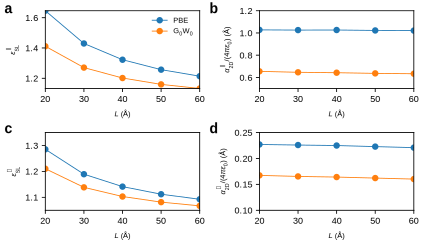
\includegraphics[width=0.9\linewidth]{img/SI-GW-alpha-zero.pdf}
 \caption{{\bf Variation of 
   $\varepsilon^{\perp}_{\mathrm{SL}}$ as a function of $L$ for
   monolayer BN calculated at the level of PBE and G$_{\rm 0}$W$_{0}$.}
   \textbf{a}-{\bf b}. $\varepsilon_{\mathrm{SL}}^{\parallel}$ and $\alpha_{\mathrm{2D}}^{\parallel}$ as function of $L$, respectively.    
  \textbf{c}-{\bf d}. $\varepsilon_{\mathrm{SL}}^{\perp}$ and 
  $\alpha_{\mathrm{2D}}^{\perp}$ as
   function of $L$. 
   In all cases the values obtained using
   G$_{0}$W$_{0}$ method is smaller than that using PBE method due to
   better estimation of the bandgap.}
  \label{fig:GW-PBE-alpha}
\end{figure}

Next we will investigate the frequency-dependent dielectric properties of the 2D materials using various methods. The imaginary part of the frequency-dependent dielectric function of an periodic system is calculated using the following relation:

\begin{equation}
\begin{aligned}
  \label{eq:dft-dielectric}
\varepsilon_{\alpha\beta}^{(2)}(\omega)=\frac{4\pi e^2}{\Omega}\lim\limits_{q\rightarrow 0}\frac{1}{q^2}\sum_{v,c,\mathbf{k}}&2\omega_\mathbf{k}\delta(\epsilon_{c\mathbf{k}}-\epsilon_{v\mathbf{k}}-\omega) \\
&\times\braket{u_{c\mathbf{k}+q\mathbf{e}_\alpha}|u_{v\mathbf{k}}}\braket{u_{v\mathbf{k}}|u_{c\mathbf{k}+q\mathbf{e}_\beta}}
\end{aligned}
\end{equation}
Through the Kramers-Kronig transformation the real part of the dielectric function can be obtained as: 

\begin{equation}
  \varepsilon_{\alpha\beta}^{(1)}(\omega)=1+\frac{2}{\pi}\int_0^\infty\frac{\varepsilon_{\alpha\beta}^{(2)}(\omega')\omega'}{\omega'^2-\omega^2}d\omega'
\end{equation}

We calculate the frequency-dependent dielectric properties of BN with
varying supperlattice $L$ at PBE, G$_{0}$W$_{0}$, and G$_{0}$W$_{0}$--BSE. 
Figure \ref{fig:PBE-omega-in} and \ref{fig:PBE-omega-out} show the
magnitudes of $\varepsilon_{\mathrm{SL}}^{\parallel}(\omega)$ and
$\varepsilon_{\mathrm{SL}}^{\perp}(\omega)$ reduce with increasing $L$
throughout the whole frequency range at PBE level. The $L$-dependency can also be
removed using Eqs. \ref{main-eq:alpha-para-def} and
\ref{main-eq:alpha-perp-def}, yielding lattice-independent
polarizabilities throughout the frequency domain (Figure \ref{fig:PBE-omega-in}{\bf b}-{\bf d} and \ref{fig:PBE-omega-out}{\bf b}-{\bf d}). 
%
Note that when extracting
the frequency-dependent 2D polarizabilities from
Eqs. \ref{main-eq:alpha-para-def} and \ref{main-eq:alpha-perp-def},
the peak position in energy $\omega (eV)$ from $\varepsilon_{\mathrm{SL}}$ is preserved. This
is explained by the fact that the local extrema from spectra of
$\varepsilon_{\mathrm{SL}}$ is also the local extrema in corresponding
$\alpha_{\mathrm{2D}}$, since when
$\partial \varepsilon_{\mathrm{SL}}(\omega) / \partial \omega = 0 $,
we have
\begin{subequations}
\begin{eqnarray}
  \label{eq:extrema-para}
  \frac{\partial \alpha_{\mathrm{2D}}^{\parallel}(\omega)}{\partial \omega}
  &= \varepsilon_{0}L {\displaystyle \frac{\partial \varepsilon_{\mathrm{SL}}^{\parallel}}{\partial \omega}} = 0   \\
  \label{eq:extrema-perp}
  \frac{\partial \alpha_{\mathrm{2D}}^{\perp}(\omega)}{\partial \omega}
  &= \varepsilon_{0}L {\displaystyle \frac{1}{\varepsilon_{\mathrm{SL}}^{2}}\frac{\partial \varepsilon_{\mathrm{SL}}^{\parallel}}{\partial \omega}} = 0
\end{eqnarray}
\end{subequations}
which indicates that no corrections in energy are present 
when transforming
$\varepsilon_{\mathrm{SL}}(\omega)$ to $\alpha_{\mathrm{2D}}(\omega)$.

We note that the result change slightly when G$_{0}$W$_{0}$ method
is used. As shown in Figures \ref{fig:GW-omega-in} and
\ref{fig:GW-omega-out}, not only do the intensity of the dielectric
functions change with $L$, but also the peak positions. As a result
the obtained polarizabilities also show $L$-dependent peak shift. This
can be explained by the long-range nature of Coulomb interactions. In
fact the self-energy of the G$_{0}$W$_{0}$ system $\Sigma$, is determined by:
\begin{equation}
  \label{eq:GW-formula}
  \Sigma = i G_{0} W_{0} = i G_{0} \varepsilon^{-1} \nu
\end{equation}
where $G$ is the non-interacting Green function, and $\nu$ is the
Coulomb interaction. Since the dielectric constant $\varepsilon$
changes with $L$, the self energy as well quasi-particle energies of
the G$_{0}$W$_{0}$ method also varies with $L$. As a result we get
higher peak energy of the dielectric spectrum when $L$ increases. Such
peculiar $L$-dependency can be minimized when adding electron-hole
interaction through the Bethe-Salpethe equation (BSE), as shown in
Figures \ref{fig:BSE-omega-in} and \ref{fig:BSE-omega-out}. The
polarizabilities again becomes lattice-independent due to the
localization of excitons within the 2D material layer, which corrects the energy shift of G$_{0}$W$_{0}$ method.



Combining the accuray of bandgap estimation, reproducible results of
frequency-dependent dielectric properties and calculation efforts, the
choice of HSE06 hybrid functional seems used in the main text provides
best tradeoff between all aspects.

\begin{figure}[htbp]
  \centering
 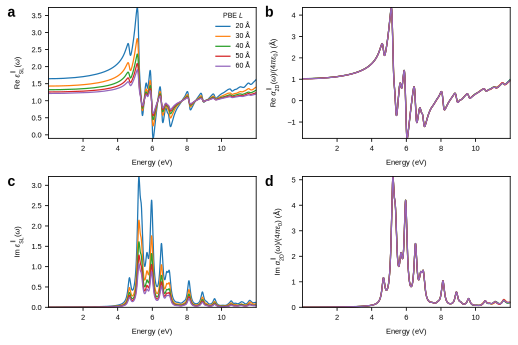
\includegraphics[width=1.00\linewidth]{img/SI-PBE-omega-in_plane.pdf}
 \caption{Dependence of in-plane dielectric properties on $L$ for
   monolayer BN calculated using PBE method: \textbf{a} Real part of
   $\varepsilon_{\mathrm{SL}}^{\parallel}$, \textbf{b} Real part of
   $\alpha_{\mathrm{2D}}^{\parallel}$, \textbf{c} Imaginary part of
   $\varepsilon_{\mathrm{SL}}^{\parallel}$, \textbf{d} Imaginary part
   of $\alpha_{\mathrm{2D}}^{\parallel}$.  The same {\bf k}-sampling
   is used in all simulations with the only variable quantity being
   $L$. Clearly, the $L$-dependency of the superlattice dielectric
   function is removed using 2D polarizabilities.}
  \label{fig:PBE-omega-in}
\end{figure}

\begin{figure}[htbp]
  \centering
  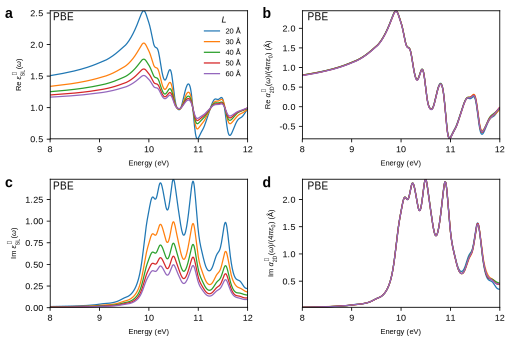
\includegraphics[width=1.0\linewidth]{img/SI-PBE-omega-out_of_plane.pdf}
  \caption{Dependence of out-of-plane dielectric properties on $L$ for
    monolayer BN calculated using PBE method: \textbf{a} Real part of
    $\varepsilon_{\mathrm{SL}}^{\perp}$, \textbf{b} Real part of
    $\alpha_{\mathrm{2D}}^{\perp}$, \textbf{c} Imaginary part of
    $\varepsilon_{\mathrm{SL}}^{\perp}$, \textbf{d} Imaginary part of
    $\alpha_{\mathrm{2D}}^{\perp}$.  The same {\bf k}-sampling is used
    in all simulations with the only variable quantity being
    $L$. Clearly, the $L$-dependency of the superlattice dielectric
    function is removed using 2D polarizabilities.}
  \label{fig:PBE-omega-out}
\end{figure}



\begin{figure}[htbp]
  \centering
 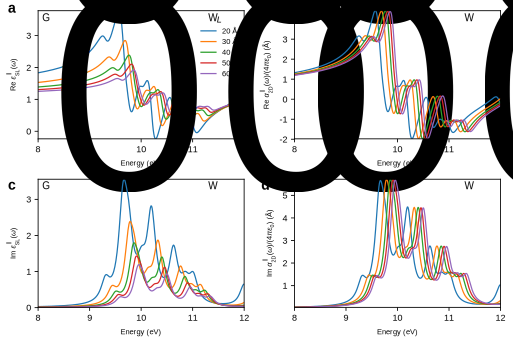
\includegraphics[width=1.0\linewidth]{img/SI-GW-omega-in_plane.pdf}
 \caption{Similar to Figure \ref{fig:PBE-omega-in} but calculated
   using G$_{0}$W$_{0}$ method. A shift of peak position (frequency)
   in the dielectric function spectra is observed, resulted from the
   change of quasi-particle energy in G$_{0}$W$_{0}$ calculations
   invloving the 2D slab.}
  \label{fig:GW-omega-in}
\end{figure}

\begin{figure}[htbp]
  \centering
 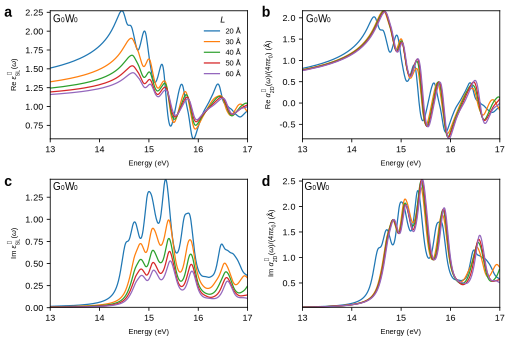
\includegraphics[width=1.0\linewidth]{img/SI-GW-omega-out_of_plane.pdf}
 \caption{Similar to Figure \ref{fig:PBE-omega-out} but calculated
   using G$_{0}$W$_{0}$ method.  A shift of peak position (frequency)
   in the dielectric function spectra is observed, resulted from the
   change of quasi-particle energy in G$_{0}$W$_{0}$ calculations
   invloving the 2D slab.}
  \label{fig:GW-omega-out}
\end{figure}


\begin{figure}[htbp]
  \centering
 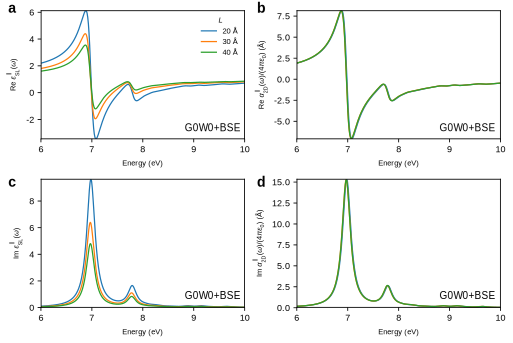
\includegraphics[width=1.0\linewidth]{img/SI-BSE-in_plane.pdf}
 \caption{Similar as in Fig. \ref{fig:GW-omega-in} but taking into
   account electron-hole interactions at the level of the
   Bethe-Salpeter equation (G$_{\rm 0}$W$_{0}$ + BSE).  The peak shift
   in energies are reduced in comparison with G$_{\rm 0}$W$_{0}$. As a
   result the polarizabilities becomes almost independent of $L$,
   consistent to results obtained by the PBE method.}
  \label{fig:BSE-omega-in}
\end{figure}

\begin{figure}[htbp]
  \centering
 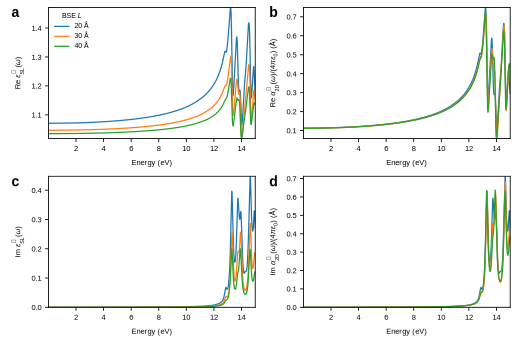
\includegraphics[width=1.0\linewidth]{img/SI-BSE-out_of_plane.pdf}
 \caption{Similar as in Fig. \ref{fig:GW-omega-out} but taking into
   account electron-hole interactions at the level of the
   Bethe-Salpeter equation (G$_{\rm 0}$W$_{0}$ + BSE).  As a result
   the polarizabilities becomes almost independent of $L$, consistent
   to results obtained by the PBE method.}
  \label{fig:BSE-omega-out}
\end{figure}

%\section{$\varepsilon^{\parallel, \perp}_{\mathrm{SL}}$ dependence on $L$}
%\label{epsilon-model}
%
%Under an external electric field $\boldsymbol{E}$ the material forming the layer 
%polarizes with a polarization $\mathcal{P}_{2D}=\chi_{2D}  \boldsymbol{E} $, where  
%$\chi_{2D} $ is the electric susceptibility of the sheet. $\mathcal{P}_{2D}$ corresponds to a dipole moment 
%in the 2D material 
%of: 
%
%\begin{equation}
%\label{P_2D}
%\boldsymbol{u}_{2D}= \mathcal{P}_{2D} \Omega = (\chi_{2D}  \boldsymbol{E}) (A L)
%\end{equation}
%\\
%From Eq. \ref{P_2D} we can calculate the dipole moment density  $\boldsymbol{\mu}_{\mathrm{2D}}^{p} =\boldsymbol{u}^{p}/A$ 

\pagebreak{}
\section{Hypothetical 2D ``dielectric constant'' rescaled from 3D dielectric constant}
\label{sec:2D-3D-rescale}
From literatures, it is often desired to extract the ``dielectric
constant'' of a 2D material from the 3D macroscopic dielectric
constant of the superlattice, where the layers are periodic along of
x,y directions but separated by a vacuum layer between its images
\cite{Matthes_2016,Laturia_2018}. As discussed in the main text, the
definition of the 2D ``dielectric constant'' (in particular, its
in-plane components) is questionable, due to the locality of
electrostatic screening of the 2D materials
\cite{Cudazzo_2010_screen2D,Cudazzo_2011_screening_2D}. Here we show
that, in addition to the ambiguous definition of the 2D dielectric
constant, such approach requires the precise determination of the 2D
layer thickness $\delta_{\mathrm{2D}}$, which makes it impractical.

In brief, the hypothetical 2D dielectric constant
$\varepsilon$ comes from the planar limit of the
Maxwell-Garnett effective medium theory \cite{Markel_2016}, and can be
expressed by means of the macroscopic dielectric constant
$\varepsilon_{\mathrm{SL}}$ of the superlattice:

\begin{eqnarray}
  \label{eq:MG-effect-1}
  &\varepsilon_{\mathrm{SL}}^{\parallel} &= f \varepsilon_{\mathrm{2D}}^{\parallel} + (1 - f)\\
  \label{eq:MG-effect-2}
  &(\varepsilon_{\mathrm{SL}}^{\perp})^{-1} &= f /\varepsilon_{\mathrm{2D}}^{\perp} + (1-f)
\end{eqnarray}
where $f=\delta/L$ is the volume fraction of the 2D
material in the superlattice and $\varepsilon_{\mathrm{2D}}^{\parallel}$ and 
$\varepsilon_{\mathrm{2D}}^{\perp}$ are the corresponding dielectric constants for the 2D layer. 
The major issue when using such rescale
relations comes from the determination of $\delta_{\mathrm{2D}}$. To
eliminate the modeling error caused by the \textit{a priori} parameter
selection of $\delta$, we perform the calculation of
$\varepsilon_{\mathrm{SL}}$ of group 6 TMDCs against different $L$,
and use least-square fitting to extract both
$\varepsilon$ and $\delta$, as shown in
Figure \ref{fig:rescale-prb}.

\begin{figure}[htbp]
  \centering
  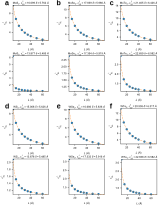
\includegraphics[width=0.85\linewidth]{img/SI-rescale-PRB.pdf}
  \caption{ Calculated (blue dots) and fitted
    (orange broken lines) $\varepsilon_{\mathrm{SL}}$ as function of
    $L$ for the group 6 TMDCs:
    \textbf{a}. MoS$_{2}$. \textbf{b}. MoSe$_{2}$. \textbf{c}.
    MoTe$_{2}$. \textbf{d}. WS$_{2}$. \textbf{e}. WSe$_{2}$. \textbf{f}.
    WTe$_{2}$. The extracted values of $\varepsilon_{\mathrm{2D}}$ and
    $\delta$ are shown in each subfigure.}
  \label{fig:rescale-prb}
\end{figure}

As can be seen from the fitted results in Figure
\ref{fig:rescale-prb}, the values of $\delta_{\mathrm{2D}}$ extracted
from both $\varepsilon_{\mathrm{SL}}^{\parallel}$ and
$\varepsilon_{\mathrm{SL}}^{\perp}$ are close when $L> 15$
{\AA}. Notably, the $\delta_{\mathrm{2D}}$ values are generally 10\%
smaller than the interlayer distance in corresponding bulk materials
$L_{\mathrm{bulk}}$ , as shown in Table \ref{tab:delta-L-DFt}. On the
other hand, the extracted $\delta_{\mathrm{2D}}$ values are closer to
the covalent thickness $\delta_{\mathrm{2D}}^{\mathrm{cov}}$ as
described in the main text, with a difference generally smaller than
5\%. Our results indicate that the conventional estimation of the 2D
layer thickness by its bulk interlayer distance
\cite{Matthes_2016,Laturia_2018}, will always lead to
overestimation. On the contrary, the out-of-plane polarizability
$\alpha_{\mathrm{2D}}^{\perp}$ correctly captures the thickness nature
of 2D materials.

\begin{table}[htbp]
  \centering
  \begin{tabular}[htbp]{lccccc}
  \hline{}
  Material & $\delta_{\mathrm{2D}}$ from $\varepsilon_{\mathrm{SL}}^{\parallel}$ ({\AA}) & $\delta_{\mathrm{2D}}$ from $\varepsilon_{\mathrm{SL}}^{\perp}$ ({\AA})& $L_{\mathrm{bulk}}$ ({\AA}) & $\delta_{\mathrm{2D}}^{\mathrm{cov}}$ ({\AA}) & $\alpha_{\mathrm{2D}}^{\perp}/\varepsilon_{0}$ ({\AA})\\
  \hline{}
  2H-MoS$_{2}$ & 5.76 & 5.49 & 6.15 & 5.22 & 4.98\\
  2H-MoSe$_{2}$ & 5.98 & 5.92 & 6.46 &  5.73 & 5.60\\
  2H-MoTe$_{2}$ & 6.43 & 6.85 & 6.98 & 6.37 & 6.12\\
  2H-WS$_{2}$ & 5.63 & 5.49 & 6.15 & 5.20 & 5.00\\
  2H-WSe$_{2}$ & 5.84 & 5.92 & 6.49 & 5.75 & 5.42\\
  2H-WTe$_{2}$ & 6.32 & 6.58 & 7.06 & 6.38 & 6.33\\
  \hline{}
\end{tabular}

\caption{Calculated $\delta_{\mathrm{2D}}$ from
  $\varepsilon_{\mathrm{SL}}^{\parallel}$ and
  $\varepsilon_{\mathrm{SL}}^{\perp}$, compared with the interlayer
  distance of corresponding bulk material $L_{\mathrm{SL}}$, the
  covalent thickness $\delta_{\mathrm{2D}}^{\mathrm{cov}}$, and
  $\alpha_{\mathrm{2D}}^{\perp}/\varepsilon_{0}$ for 2H TMDC materials.}
\label{tab:delta-L-DFt}
\end{table}

Another drawback of the 2D dielectric constant approach is the
overestimation of the out-of-plane dielectric response. As can be seen
in Figure \ref{fig:rescale-prb}, the extracted
$\varepsilon_{\mathrm{2D}}^{\perp}$ values for the TMDCs studied
are comparable or even larger than
$\varepsilon_{\mathrm{2D}}^{\parallel}$, which does not agree with the
physical picture that electrostatic screening of 2D materials are much
smaller perpendicular to the 2D plane. In fact, combining
Eq. \ref{eq:MG-effect-1} and the definition of $\alpha_{\mathrm{2D}}^{\perp}$, we
have:
\begin{equation}
  \label{eq:eps-alpha-perp}
  \frac{\alpha_{\mathrm{2D}}^{\perp}}{\varepsilon_{0}} = \delta_{\mathrm{2D}}(1 - (\varepsilon_{\mathrm{2D}}^{\perp})^{-1})
\end{equation}

\begin{figure}[htbp]
  \centering
  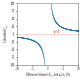
\includegraphics[width=0.6\linewidth]{img/SI-eps-alpha-error.pdf}
  \caption{Calculated $\varepsilon_{\mathrm{2D}}^{\perp}$ value as a
    function of the difference between $\delta_{\mathrm{2D}}$ and
    $\alpha_{\mathrm{2D}}^{\perp}/\varepsilon_{0}$. A small change of
    $\alpha_{\mathrm{2D}}^{\perp}/\varepsilon_{0}$ chosen may lead to divergence of
    the $\varepsilon_{\mathrm{2D}}^{\perp}$ or even negative values,
    which is apparently unphysical}
  \label{fig:eps-alpha-error}
\end{figure}

which indicate that the characteristic length
$\alpha_{\mathrm{2D}}^{\perp}/\varepsilon_{0}$, is very close but slightly smaller
than $\delta_{\mathrm{2D}}$ estimated by the effective medium theory,
if $\varepsilon^{\perp}_{\mathrm{2D}} \gg 1$. Moreover, from
Eq. \ref{eq:eps-alpha-perp}, when $\delta_{\mathrm{2D}}$ and
$\alpha_{\mathrm{2D}}^{\perp}/\varepsilon_{0}$ are close, slight change of the
$\delta_{\mathrm{2D}}$ chosen may lead to divergence of
$\varepsilon_{\mathrm{2D}}^{\perp}$, as shown in Figure
\ref{fig:eps-alpha-error}. Therefore cautions must to taken when
treating the dielectric response of the 2D material using effective
medium theory. In comparison, the 2D polarizability does not require
the guess of the thickness, and therefore is the true descriptor of
the 2D dielectric nature.

To conclude, based on theoretical and technical considerations, there are several
advantages of using the polarizability $\alpha$ for describing the dielectric
nature of 2D materials, including
\begin{enumerate}
\item $\alpha_{\mathrm{2D}}$ can be used to describe both the local and macroscopic dielectric properties, while $\epsilon_{\mathrm{2D}}$ can't.
\item Calculating $\alpha_{\mathrm{2D}}$ only requires to calculate the dielectric response at single superlattice length, while $\epsilon_{\mathrm{2D}}$ requires calculation with varied superlattice length.
\item $\alpha_{\mathrm{2D}}$ correctly represents the screening length of 2D material, while $\epsilon_{\mathrm{2D}}$ does not.
\item $\alpha_{\mathrm{2D}}$ correctly represents the different degree of screening in/out-of-plane, while $\epsilon_{\mathrm{2D}}$ does not.
  
\item The value of $\epsilon_{\mathrm{2D}}$ hugely depends on the
  choice of the thickness of 2D material, while such information is
  intrinsically embedded in $\alpha_{\mathrm{2D}}$.
\end{enumerate}


%%%%%%\section{Theoretical Analysis}
%%%%%%\label{sec:theory}
\section{Polarizability-Based Theoretical Model}
\label{sec:theory-1}
The universal relations for $\alpha_{\mathrm{2D}}^{\parallel}$ and
$\alpha_{\mathrm{2D}}^{\perp}$ revealed by main text
Eqs. \ref{main-eq:2D-Moss-para} and \ref{main-eq:2D-Moss-perp} are not
coincidental. Combining recent theoretical findings of the linear
relation between exciton binding energy $E_{\mathrm{b}}$ and
$E_{\mathrm{g}}$ of 2D materials
\cite{Choi_linear_2015,Olsen_2016_hydrogen,Jiang_2017_Eg_Eb}, and the
fact that the $E_{\mathrm{b}}$ is roughly inversely proportional to
$\alpha_{\mathrm{2D}}^{\parallel}$ \cite{Pulci_2014}, it is reasonable
to have a general relation between
$\alpha_{\mathrm{2D}}^{\parallel}$ and $E_{\mathrm{g}}^{-1}$. Moreover,
the bandgap-independent relation of 2D $\alpha_{\mathrm{2D}}^{\perp}$
resembles molecular polarizabilities of conjugate molecules
\cite{Davies_1952}, fullerenes \cite{Sabirov_2014} and carbon
nanotubes \cite{Benedict_1995}, which are also shown to be
geometry-dependent.

In this section we show in detail the polarizability-based theoretical
framework that leads to the 2D Moss-like relations proposed in the
main text.  Due to its highly anisotropic nature, the wave function of
an isolated 2D material $\psi(\mathbf{r})$ can be separated into the
in- and out-of-plane components ($\psi^{\parallel}(\boldsymbol{\rho})$ and $\psi^{\perp}(z)$) 
similar to the treatment of quantum
wells (QW),\cite{davies_physics_1997} such that
$\psi=\psi^{\parallel}\psi^{\perp}$, where $\boldsymbol{\rho}=(x, y)$
is the in-plane coordinate. Using the Bloch theorem, the periodic
$\psi^{\parallel}(\boldsymbol{\rho})$ can be further expressed as
$\psi^{\parallel}(\boldsymbol{\rho})=e^{i\mathbf{k} \cdot
  \boldsymbol{\rho}}u(\boldsymbol{\rho})$, where $\mathbf{k}$ is the
in-plane wave vector and $u(\boldsymbol{\rho})$ is periodic function
in the xy-plane. According to the random phase approximation (RPA)
theory\cite{Adler_1962}, $\varepsilon_{\mathrm{SL}}$ is the
$\mathbf{q} \to 0$ and $\omega \to 0$ limits of the non-interacting
dielectric function $\varepsilon(\mathbf{q}, \omega)$, where
$\mathbf{q}$ is the momentum transfer and $\omega$ is the frequency:
\begin{equation}
  \label{eq:RPA-eps2}
  \varepsilon_{\mathrm{SL}}
  = \lim_{\mathbf{q} \to 0} 1 + \frac{2e^{2}}{\varepsilon_{0} |\mathbf{q}|^{2} \Omega}
  \sum_{\mathrm{k, c, v}}
  \frac{|<\psi_{\mathrm{v}}(\mathbf{k})|e^{-i\mathbf{q}\mathbf{r}}|\psi_{\mathrm{c}}(\mathbf{k+q})>|^{2}}
  {E_{\mathrm{c}}(\mathbf{k+q}) - E_{\mathrm{v}}(\mathbf{k})}
  \left[f(\psi_{\mathrm{c}}) - f(\psi_{\mathrm{v}})\right]
\end{equation}
where $e$ is the unit charge, $c$, $v$ are the conduction and valence
bands, $E$ is the eigenenergy of individual bands, and $f$ is the
Fermi-Dirac distribution function. Taking the
limit that $L\to\infty$, when
$\varepsilon^{\perp}_{\mathrm{SL}} \approx 1$, we have
$1-1/\varepsilon^{\perp}_{\mathrm{SL}} \approx
(\varepsilon_{\mathrm{SL}}^{\perp} - 1)$. Therefore
$\alpha_{\mathrm{2D}}^{\parallel}$ and $\alpha_{\mathrm{2D}}^{\perp}$
at 0 K can be unified by the same equation:
\begin{equation}
  \label{eq:alpha-RPA}
  \alpha = \frac{2e^{2}}{|q|^{2}A} \sum_{\mathrm{k,c,v}}
  \frac{|<\psi_{\mathrm{v}}(\mathbf{k})|e^{-i\mathbf{q}\mathbf{r}}|\psi_{\mathrm{c}}(\mathbf{k+q})>|^{2}}
  {E_{\mathrm{c}}(\mathbf{k+q}) - E_{\mathrm{v}}(\mathbf{k})}
\end{equation}
where the direction is determined by $\mathbf{q}$. Next we will show
that the different behavior of $\psi^{\parallel}$ and $\psi^{\perp}$
give rise to the main text Eqs. \ref{main-eq:2D-Moss-para} and
\ref{main-eq:2D-Moss-perp}.

% {\bf ES:} There is something weird with the cross-referencing for the equations 3a and 3b between the main text and 
% SI. They changed to 2a and 2b in the SI. 


\subsection{Detailed derivations of Eq. \ref{main-eq:2D-Moss-para}}  %
\label{ssec:theory-1-para}

In this section we show how Eq. \ref{main-eq:alpha-para-def}
is derived from Eq. \ref{eq:alpha-RPA}. For the in-plane component
$\alpha_{\mathrm{2D}}^{\parallel}$, $e^{-i\mathbf{qr}}$ is independent
of $z$, therefore the integral in
$|<\psi_{\mathrm{v}}(\mathbf{k})|e^{-i\mathbf{q}\mathbf{r}}|\psi_{\mathrm{c}}(\mathbf{k+q})>|^{2}$
becomes independent of $\psi^{\perp}$, due to the orthogonality
and normality. The Bloch-wave form of $\psi^{\parallel}$ ensures that
only the cell-function $u(\mathbf{k})$ contributes to the final result
of $\alpha^{\parallel}_{\mathrm{2D}}$ \cite{davies_physics_1997}, such
that:
\begin{equation}
  \label{eq:alpha_para_RPA}
  \alpha_{\mathrm{2D}}^{\parallel} = \frac{2e^{2}}
  {(2 \pi)^{2}} \int d^{2}\mathbf{k} \sum_{\mathrm{c, v}}
  \frac{|<u_{\mathrm{c}}(\mathbf{k})|\nabla|u_{\mathrm{v}}(\mathbf{k})>|^{2}}
  {E_{\mathrm{c}}(\mathbf{k}) - E_{\mathrm{v}}(\mathbf{k})}
\end{equation}
Following the method of $\mathbf{k} \cdot \mathbf{p}$ theory from
Ref. \citenum{Jiang_2017_Eg_Eb}, the matrix element in the numerator
of Eq. \ref{eq:alpha_para_RPA} is approximated by:

\begin{equation}
\label{eq:matrix-approx}
|<u_{\mathrm{c}}(\mathbf{k})|\nabla|u_{\mathrm{v}}(\mathbf{k})>|^{2}
\approx {\displaystyle \frac{\hbar^{2}}{2 m^{*}}
  \frac{1}{E_{\mathrm{g}} + \frac{\hbar^{2} k^{2}}{2 m^{*}}}}
\end{equation}
plug it into Eq. \ref{eq:alpha_para_RPA} and integrate within the 2D Brillouin zone from $|k|=0$ to $|k|= k_{\mathrm{BZ}}$, where $k_{\mathrm{BZ}}$ is the wavevector at the boundary of the 2D Brillouin Zone, we get:
\begin{equation}
  \label{eq:derivation-2D-Moss-para}
  \begin{aligned}
\alpha_{\mathrm{2D}}^{\parallel} &= N\cdot -\frac{e^{2}}{2 \pi}
\frac{1}{E_{g} + \beta} \Biggr\vert_{\beta=0}^{\beta=\frac{\hbar^{2} k^{2}_{\mathrm{BZ}}}{m^{*}}} \\
&\approx N e^{2}/(2\pi E_{\mathrm{g}}) = C^{\parallel} E_{g}^{-1}
\end{aligned}
\end{equation}
where $N$ is de degeneracy of bands associated with $E_{g}$. The
approximation in Eq. \ref{eq:derivation-2D-Moss-para} is due to the
fact that $\frac{\hbar^{2} k^{2}_{\mathrm{BZ}}}{m^{*}} \gg E_{g}$, and
we arrive at Eq. \ref{main-eq:2D-Moss-para}.

The coefficient of $C^{\parallel}$ adapted from
Ref. \citenum{Jiang_2017_Eg_Eb} $C^{\parallel} = N e^{2}/(2\pi)$
predicts linear correlation between $\alpha^{\parallel}_{\mathrm{2D}}$
and $E_{\mathrm{g}}^{-1}$. We validate this by examining the
DFT-calculated
$(4\pi \varepsilon_{0})/\alpha^{\parallel}_{\mathrm{2D}}$ (measured in
\AA{}$^{-1}$) and $E_{\mathrm{g}}$ (measured in eV) in
Figure \ref{main-fig-3}\textbf{c}. The coefficient $C^{\parallel}$
becomes
$8 \pi^{2} \varepsilon_{0} \AA{} / (e N) \approx 0.436 / N = 0.183$,
corresponding to $N$ between 2 and 3, which is a reasonable result for
the 2D materials studied.

% {\bf ES:} Tian, please include more details in this section on the derivations! 


\subsection{Detailed derivation of Eq. \ref{main-eq:2D-Moss-perp}}
\label{ssec:theory-1-perp}

For Eq. \ref{main-eq:2D-Moss-perp}, treating the in-plane
wave functions as plane wave with form
$\psi^{\parallel}(\rho) \propto e^{i \mathbf{k \rho}}$, the matrix
element of
$<\psi_{\mathrm{v}}(\mathbf{k})|e^{-i\mathbf{qr}}|\psi_{\mathrm{c}}(\mathbf{k+q})>$,
when $\mathbf{q}=(0, 0, q_{z})$, becomes\cite{Hybertsen_1987}:
\begin{equation}
  \begin{aligned}
    \label{eq:matrix-z}
  <\psi_{\mathrm{v}}(\mathbf{k})|e^{-i\mathbf{qr}}|\psi_{\mathrm{c}}(\mathbf{k+q})>
  &= \frac{1}{A} \int dx \int dy
  e^{i(\mathbf{-k \rho} - \mathbf{q \rho} + \mathbf{(k+q) \rho})}
  \int (\psi^{\perp})^{*}_{\mathrm{v}}(\mathbf{k})e^{-iq_{z}z}\psi^{\perp}_{\mathrm{c}}(\mathbf{k+q})\\
  &= <\psi^{\perp}_{\mathrm{v}}(\mathbf{k})|e^{-iq_{z}z}|\psi^{\perp}_{\mathrm{c}}(\mathbf{k+q})>
  \end{aligned}
\end{equation}
Note that the states perpendicular are bound, the integral is
meaningful only when $\mathbf{k=k+q}$ \cite{davies_physics_1997}. By
performing the Taylor expansion of
$e^{-i\mathbf{qr}} \approx 1 - i\mathbf{qr}$, we get:
\begin{equation}
  \begin{aligned}
    \label{eq:matrix-z-2}
    <\psi^{\perp}_{\mathrm{v}}(\mathbf{k})|e^{-iq_{z}z}|\psi^{\perp}_{\mathrm{c}}(\mathbf{k})>
    &\approx <\psi^{\perp}_{\mathrm{v}}(\mathbf{k})|\psi^{\perp}_{\mathrm{c}}(\mathbf{k})> -
    iq_{z} <\psi^{\perp}_{\mathrm{v}}(\mathbf{k})|z|\psi^{\perp}_{\mathrm{c}}(\mathbf{k})>\\
    &= -iq_{z} <\psi^{\perp}_{\mathrm{v}}(\mathbf{k})|z|\psi^{\perp}_{\mathrm{c}}(\mathbf{k})>
   \end{aligned}
\end{equation}
plug this into Eq. \ref{eq:alpha-RPA} and express the summation over
$k_{x}$ and $k_{y}$ in a continuous form within the Brillouin Zone, we
arrive at:
\begin{equation}
\label{eq:alpha_perp_RPA}
\alpha_{\mathrm{2D}}^{\perp} = \frac{2e^{2}}{(2 \pi) ^{2}} \int d^{2}\mathbf{k}
\sum_{\mathrm{c, v}}
\frac{|<\psi_{\mathrm{v}}(\mathbf{k})|z|\psi_{\mathrm{c}}(\mathbf{k})>|^{2}}
{E_{\mathrm{c}}(\mathbf{k}) - E_{\mathrm{v}}(\mathbf{k})}
\end{equation}
The formalism is slightly different from Eq.\ref{eq:alpha_para_RPA}.

The out-of-plane wave function $\psi^{\perp}(z)$ is the solution to the Schr\"{o}dinger equation with
Hamiltonian $\mathcal{H} = -\hbar^{2} \nabla^{2}/2m_{e} + V(z)$, where
$\hbar$ is the reduced Planck constant, $m_{e}$ is electron mass and
$V(z)$ is the confined Coulomb potential along the z-direction
created by the nuclei
\cite{davies_physics_1997,ihn_semiconductor_2009}. Although the exact
form for $\psi^{\perp}$ depends on the exact distribution of $V(z)$,
without loss of generality we can assume the electrons are confined in
a potential well of width $\delta$, which is the typical treatment for
semiconductor QWs \cite{ihn_semiconductor_2009,Fowler_1984,Maize_2011}. 
The allowed bound
states inside the confined region generally have wave vector
$k_{z} \propto n \pi / \delta$. With the total energy
$E_{n}(\mathbf{k}) = {\displaystyle \frac{\hbar^{2} (k_{x}^{2} +
    k_{y}^{2})}{2 m^{\parallel}} + \frac{\hbar^{2} n^{2} \pi^{2}}{2
    m^{\perp} \delta^{2}}}$, where $m^{\parallel}$ and $m^{\perp}$ are
the effective masses parallel and perpendicular to the 2D
plane. Therefore, the denominator of Eq. \ref{eq:alpha_perp_RPA} becomes independent of
$\mathbf{k}$, that
$E_{\mathrm{c}}(\mathbf{k}) - E_{\mathrm{v}}(\mathbf{k}) =
(n_{\mathrm{c}}^{2} - n_{\mathrm{v}}^{2}) {\displaystyle
  \frac{\hbar^{2} \pi^{2}}{2 m^{\perp} \delta^{2}}}$. On the other
hand, the numerator
$<\psi^{\perp}_{\mathrm{v}}(\mathbf{k})|z|\psi^{\perp}_{\mathrm{c}}(\mathbf{k})>$
is proportional to the confinement length $\delta$ which can be seen using the 
particle-in-box solution\cite{davies_physics_1997}. In combination,
the individual terms of the summation in the right hand of Eq. \ref{eq:alpha_perp_RPA} is
independent of neither $E_{\mathrm{g}}$ nor \textbf{k}, proving that
$\alpha_{\mathrm{2D}}^{\perp}$ is independent of the band gap.
%
%Finally we will show the $\alpha_{\mathrm{2D}}^{\perp}$ is related to the
%confinement length $\delta$, or equivalently the thickness of the 2D
%material. For simplicity we assume $\psi^{\parallel}$ is the solution
%of a particle confined inside an infinite potential well of width
%$\delta$ with the form $\psi \propto \sin(\frac{n\pi}{\delta})$. At 0
%K, the only non-zero contribution for the transition between band
%$n_{\mathrm{v}}$ and $n_{\mathrm{c}}$ corresponds with in-plane wave
%vector $\mathbf{k}_{\rho}$ within the range of $k_{\mathrm{F}}^{\mathrm{v}}$ to
%$k_{\mathrm{F}}^{\mathrm{c}}$, the Fermi vectors of each band. Therefore we have:
%\begin{equation}
%  \begin{aligned}
%    \alpha_{\mathrm{2D}}^{\perp} &\propto \delta^{4} m^{\perp} \int
%    d^{2}\mathbf{k}_{\rho}
%    \frac{f(\psi_{\mathrm{v}}(\mathbf{k}_{\rho}))
%      -f(\psi_{\mathrm{v}}(\mathbf{k}_{\rho})) }{n_{\mathrm{c}}^{2} -
%      n_{\mathrm{v}}^{2}}\\
%    &= \delta^{4} m^{\perp} \sum_{\mathrm{c, v}}\pi \frac{
%      (k_{\mathrm{F}}^{\mathrm{c}})^{2} -
%        (k_{\mathrm{F}}^{\mathrm{v}})^{2}}{n_{\mathrm{c}}^{2} -
%        n_{\mathrm{v}}^{2}}
%  \end{aligned}
%\end{equation}
%Since the Fermi wave vector for band \textit{i} follows
%${\displaystyle
%  \frac{\hbar^{2}(k_{\mathrm{F}}^{i})^{2}}{2m^{\parallel}}} +
%{\displaystyle \frac{\hbar^{2} n_{i}^{2} \pi^{2}}{2m^{\perp}
%    \delta^{2}}} = E_{\mathrm{F}}$, we have
%$ (k_{\mathrm{F}}^{\mathrm{c}})^{2} -
%(k_{\mathrm{F}}^{\mathrm{v}})^{2} \propto (n_{\mathrm{c}}^{2} -
%n_{\mathrm{v}}^{2}) {\displaystyle
%  \frac{m^{\parallel}}{m^{\perp}}}$. Note that in the particle-in-box
%model, the energy levels for a sub-nm QW will be at the order of 10
%eV, which allows only few states inside the QW. Combine with the fact
%that the strongest transition mostly comes from the lowest bands
%\cite{davies_physics_1997}, $\alpha^{\perp}_{\mathrm{2D}}$ is shown to
%be proportional to $\delta^{p}$, where the power index $p$ is 2. We
%note the different power law comes from the choice of the $V(z)$. The
%atomic polarizabilities of free particles inside a 1D infinite QW,
%finite QW or harmonic QW all show dependency with $\delta^{4}$, where
%$\delta$ is the length of confinement or effective harmonic length of
%the QW \cite{Fowler_1984,Maize_2011}. Since the 2D polarizability is
%the molecular polarizability divided by the area, such approach will
%always yield $\alpha_{\mathrm{2D}}^{\perp} \propto \delta^{2}$. To
%accurately model the $\alpha_{\mathrm{2D}}^{\perp}$ we need a better
%model for the confinement in z-direction than simple square potential
%well, which may be explored further. Nevertheless the simple model
%presented here still captures the bandgap-independent and
%thickness-related feature of $\alpha_{\mathrm{2D}}^{\perp}$,
%supporting our findings in the main text. 
In the next section we will
provide a simple explanation for the $\alpha \propto \delta$ relation
from fundamental electrostatics theory.

\subsection{Explanation of Eq. \ref{main-eq:2D-Moss-perp}
  from fundamental electrostatics}
\label{ssec:theory-1-perp-fundamental}

The dependency of $\alpha_{\mathrm{2D}}^{\perp}$ on the thickness
$\delta$ of a 2D material, can also be regarded using fundamental
electrostatic model. Consider the smallest repeating unit of the 2D
material with xy-plane area $A$, under small perturbation field $E$
along the z-direction.  Note that the surface bound charge
$\sigma_{\mathrm{b}}=n e /A$, where $n$ is the number of unit charges
contributes to the bound charges, comes only from the dipoles of the
outer-most atoms, since the induced charges from inner atoms are
cancel out (see Figure \ref{fig:classic-model}).
\begin{figure}[htbp]
  \centering
  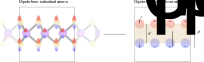
\includegraphics[width=0.99\linewidth]{img/SI-classic.pdf}
  \caption{Fundamental electrostatic model for the
    thickness-dependency of $\alpha_{\mathrm{2D}}^{\perp}$, using 2H-MoS2 as an
    example. Left: induced dipoles from individual atoms along the
    z-direction. The positive and negative induced charges from inner
    atoms cancel out. Right: simplified model for the thickness
    dependency of $\alpha_{\mathrm{2D}}^{\perp}$, where the surface dipole density
    $\boldsymbol{\mu}$ comes only from the outer-most atoms.}
  \label{fig:classic-model}
\end{figure}
From the definition of
$\alpha_{\mathrm{2D}}^{\perp}$, we have:
\begin{equation}
  \label{eq:alpha-classic}
  \alpha_{\mathrm{2D}}^{\perp} = \frac{\boldsymbol{u}_{z}}{E_{\mathrm{loc}} A}
  = \frac{(d_{\mathrm{max}} + r_{\mathrm{cov}}^{i} + r_{\mathrm{cov}}^{j}) \sigma_{\mathrm{b}}}{E}
\end{equation}
where $r_{\mathrm{cov}}^{i}$ and $r_{\mathrm{cov}}^{j}$ are the
covalent radii of the outer-most atoms, the characteristic length of
the dipole extension in z-direction, respectively, and $d_{\mathrm{max}}$ is the
z-distance between the nuclei of such atoms.  The field $E$
counterbalances the field from the surface bound charges and equals
$E = \sigma_{\mathrm{b}}/\varepsilon_{0}$. Therefore we have:
\begin{equation}
  \label{eq:alpha-classic-2}
  \alpha_{\mathrm{2D}}^{\perp} = (d_{\mathrm{max}} + r_{\mathrm{cov}}^{i} + r_{\mathrm{cov}}^{j})\varepsilon_{0}
                = \delta_{\mathrm{cov}} \varepsilon_{0}
\end{equation}
which explains the linear relation seen in Figure
\ref{main-fig-3}d. We can see that such simple model nicely captures
the thickness feature of $\alpha_{\mathrm{2D}}^{\perp}$, and
reproduces the right coefficient between $\delta_{\mathrm{cov}}$ and
$\alpha_{\mathrm{2D}}^{\perp}$.


\section{Dependence of $\alpha_{\mathrm{2D}}$ on bandgap}
\label{sec:pol-2D-Eg}

In this section we further look into the bandgap dependency of the 2D
polarizability. Figure \ref{fig:SI-raw-HSE} shows the raw data of
$\alpha_{\mathrm{2D}}^{\parallel}$ and $\alpha_{\mathrm{2D}}^{\perp}$
as functions of $E_{\mathrm{g}}$ of the 2D materials investigated. We
observe that $\alpha_{\mathrm{2D}}^{\parallel}$ can be approximated by
a reciprocal function of $E_{\mathrm{g}}$, that
$\alpha_{\mathrm{2D}}^{\parallel}\sim{}
7.295(E_{\mathrm{g}})^{-1}$. On the other hand, the plot of
$\alpha_{\mathrm{2D}}^{\perp}$ against $E_{\mathrm{g}}$ shows no
apparent correlation.
\begin{figure}[htbp]
  \centering
  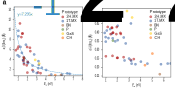
\includegraphics[width=0.99\linewidth]{img/SI-alpha_EG_raw_HSE.pdf}
  \caption{$E_{\mathrm{g}}$-dependence of \textbf{a,} $\alpha_{\mathrm{2D}}^{\parallel}$ and
    \textbf{b,} $\alpha_{\mathrm{2D}}^{\perp}$ for the 2D materials investigated here using HSE06.}
  \label{fig:SI-raw-HSE}
\end{figure}

\begin{figure}[htbp]
  \centering
  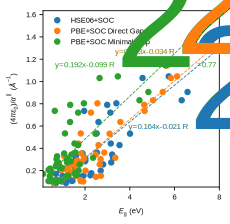
\includegraphics[width=0.6\linewidth]{img/SI-compare_alpha_Eg.pdf}
  \caption{Relation between $1/\alpha_{\mathrm{2D}}^{\parallel}$ and various choices
    of $E_{\mathrm{g}}$: minimal gap from HSE06 (blue), minimal gap
    from PBE (orange) and direct gap from PBE (green). The linear
    regression results are shown as broken lines.}
  \label{fig:alpha-Eg-diff}
\end{figure}

We also investigate the relation of 2D polarizabilities with
difference choices of \textit{ab initio} bandgaps. It is widely
accepted that the PBE exchange correlation, tends to underestimate the
bangap \cite{Heyd_2005,Kumar_2016_PRB,Kumar_2016_jpcc}.  Indeed,
changing the choice of $E_{\mathrm{g}}$ yields different regression
relation with $1/\alpha_{\mathrm{2D}}^{\parallel}$, as shown in Figure
\ref{fig:alpha-Eg-diff}. We see that due to the underestimation of PBE
bandgap, the slope of linear regression is larger than that from
HSE-bandgap. We also observe that the $1/\alpha-E_{\mathrm{g}}$
relation is better presented by using the minimal HSE bandgap than the
minimal PBE bandgap, due to higher regression $R^{2}$ coefficient of
the former. We note that the higher $R^{2}$ coefficient observed using
the direct PBE bandgap than the minimal PBE bandgap may be solely
caused by the fact that the direct bandgap of 2D materials on the PBE
level is closer to the HSE bandgap. From the random phase
approximation theory of dielectric response, the polarizability is
contributed by all possible transition between valence and conduction
bands, with the minimal bandgap as the least possible transition. In
this sense, $\alpha_{\mathrm{2D}}^{\parallel}$ is mostly like to be associated with
the minimal, not direct bandgap, as also observed in the original Moss
relation. We also examine the validity of such statement based on the
analysis of a different database\cite{Haastrup_2018} 
as will be discussed in the following sections.


\section{Using a different dataset of 2D materials}
\label{sec:gpaw}
\subsection{Validation of the universal description of 2D polarizabilities}
\label{sec:gpaw-1}

\begin{figure}[htbp]
  \centering
  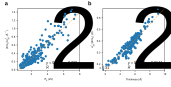
\includegraphics[width=1.05\linewidth]{img/SI-gpaw-data.pdf}
  \caption{Validation of the linear relation between \textbf{a,}
    $1/\alpha_{\mathrm{2D}}^{\parallel}-E_{\mathrm{g}}(\mathrm{HSE})$
    and \textbf{b,}
    $\alpha_{\mathrm{2D}}^{\perp}-\delta_{\mathrm{cov}}$ from 
    Ref.\cite{Haastrup_2018} corresponding to Figure \ref{main-fig-3}{\bf c}
    and \ref{main-fig-3}{\bf d}.}
  \label{fig:gpaw-alpha-relation}
\end{figure}

Due to time-consuming simulations and significant increment in 
memory overload, high-accurate calculations at hybrid HSE06 level is limited 
to about 56 compounds. 
It is desirable to validate our proposed
relations on an even larger scale database. We select over 230
semiconducting 2D materials from Ref.\cite{Haastrup_2018} 
with a GW bandgap
larger than 0.05 eV and extracted the 2D polarizabilities calculated
on the PBE level. The proposed linear relations between
$1/\alpha_{\mathrm{2D}}^{\parallel}-E_{\mathrm{g}}(\mathrm{HSE})$ and
$\alpha_{\mathrm{2D}}^{\perp}-\delta_{\mathrm{cov}}$ are also valid,
as shown in Figure \ref{fig:gpaw-alpha-relation}. Excellent linear
correlation is observed in both cases with the $R^{2}$ coefficient
larger than 0.9 which indicates the existence of a universal description 
of 2D dielectric nature through the proposed relations with the 2D
polarizabilities. We note that the slope of the linear regression is
slightly different from the one proposed from the dielectric
response at the HSE06 level. 

\subsection{Choice of bandgap}
\label{sec:gpaw-2}

Next we investigate the influence of choice of $E_{\mathrm{g}}$ on the
regression of $\alpha_{\mathrm{2D}}^{\parallel}-E_{\mathrm{g}}$ relation. Figure
\ref{fig:SI-gpaw-alpha-Eg-all} shows $1/\alpha_{\mathrm{2D}}^{\parallel}$ from 
Ref.\cite{Haastrup_2018} as a function of minimal and direct bandgap calculated
on PBE, HSE06 and GW levels. We observe,
although the regression $R^{2}$ coefficient in all cases are around
0.9, the $\alpha_{\mathrm{2D}}^{\parallel}-E_{\mathrm{g}}$ is better described using
the HSE and GW bandgaps than the PBE bandgaps. On the other hand,
using indirect or minimal bandgaps on the same level gives almost
identical regression slope. The observations are in good agreement
with our calculations on the HSE level discussed in Section
\ref{sec:pol-2D-Eg}. In combination with the physical contribution of
$E_{\mathrm{g}}$ to the dielectric screening, we conclude that the
minimal bandgap should be used for quantitative prediction of the
in-plane 2D polarizability. The prediction is greatly improved when
more accurate theory level for bandgap is used (for instance, HSE and GW).

\begin{figure}[htbp]
  \centering
  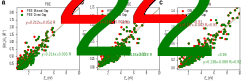
\includegraphics[width=1.05\linewidth]{img/SI-gpaw-alpha_Eg_all.pdf}
  \caption{$\alpha_{\mathrm{2D}}^{\parallel}$ as function of minimal and direct
    $E_{\mathrm{g}}$ calculated on different theoretical levels:
    \textbf{a,} PBE, \textbf{b,} HSE and \textbf{c,} GW of Ref.\cite{Haastrup_2018}.}
  \label{fig:SI-gpaw-alpha-Eg-all}
\end{figure}

For 2D materials, the exciton effect plays an important role in
determining the experimentally accessible bandgap
\cite{Arnaud_2006_exc_hBN,Pulci_2014,Ramasubramaniam_2012,Chernikov_2014_EB_MoS2_2D3D}. The
experimentally observed optical bandgap
$E_{\mathrm{g}}^{\mathrm{opt}}$, is usually lower than the direct
bandgap from band structure $E_{\mathrm{g}}^{\mathrm{dir}}$ by the
exciton binding energy $E_{\mathrm{b}}$, which is at the 10$^{-1}$ to
10$^{1}$ eV for different 2D materials due to the attenuated
dielectric screening. Next we examine the relation between
$\alpha_{\mathrm{2D}}^{\parallel}$ and $E_{\mathrm{g}}^{\mathrm{opt}}$
from Ref.\cite{Haastrup_2018} with
$E_{\mathrm{g}}^{\mathrm{opt}}=E_{\mathrm{g}}^{\mathrm{dir,QP}}-E_{\mathrm{b}}^{\mathrm{BSE}}$,
where $E_{\mathrm{g}}^{\mathrm{dir,QP}}$ is the direct quasi-particle
bandgap calculated using G$_0$W$_0$ method and
$E_{\mathrm{b}}^{\mathrm{BSE}}$ is the exciton binding energy
calculated using the Bethe-Salpethe equation. Figure \ref{fig:opt}
shows $(4\pi\varepsilon_{0})/\alpha_{\mathrm{2D}}^{\parallel}$ as a
function of $E_{\mathrm{g}}^{\mathrm{opt}}$, with a linear regression
slope of 0.154 and $R^{2}$ of 0.84, similar to the relation between
$(4\pi \varepsilon_{0})/\alpha_{\mathrm{2D}}^{\parallel}$ and
$E_{\mathrm{g}}$ (from HSE06 level, see Figures \ref{fig:SI-raw-HSE}
and \ref{fig:SI-gpaw-alpha-Eg-all}). The roughly linear correlation
between $(4\pi \varepsilon_{0})/\alpha_{\mathrm{2D}}^{\parallel}$ and
$E_{\mathrm{g}}^{\mathrm{opt}}$ is not coincidental: in fact,
theoretical analysis shows that the binding energy $E_{\mathrm{b}}$ is
proportional to the direct bandgap $E_{\mathrm{g}}$
\cite{Jiang_2017_Eg_Eb}, taking into account that
$(\alpha_{\mathrm{2D}}^{\parallel})^{-1} \propto E_{\mathrm{g}}$, we
rationalize that
$(\alpha_{\mathrm{2D}}^{\parallel})^{-1} \propto
E_{\mathrm{g}}^{\mathrm{opt}}=E_{\mathrm{g}}^{\mathrm{dir}}-E_{\mathrm{b}}$. The
slightly smaller linearity than the 2D Moss-like relation is caused
from multiple approximations used. Nevertheless we show that
$(4\pi\varepsilon_{0})/\alpha_{\mathrm{2D}}^{\parallel}$ can be
equivalently predicted using the experimentally accessible optical
bandgap.

\begin{figure}[htbp]
  \centering
  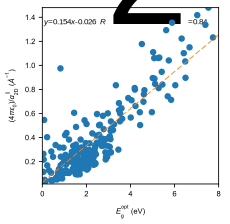
\includegraphics[width=0.70\linewidth]{img/SI-alphax-Eg-opt.pdf}
  \caption{$(4\pi\varepsilon_{0})/\alpha_{\mathrm{2D}}^{\parallel}$ as a function of
    $E_{\mathrm{g}}^{\mathrm{opt}}$ from Ref.\cite{Haastrup_2018}.}
  \label{fig:opt}
\end{figure}

\subsection{Relation between 2D polarizabilities and other physical quantities}
\label{sec:gpaw-3}

The relatively large size of Ref.\cite{Haastrup_2018} database allows us
to examine the relation between 2D polarizabilities and other physical
quantities. We choose the following quantities for comparison,
corresponding to Figures \ref{fig:gpaw-2D-quantities-1} to
\ref{fig:gpaw-2D-quantities-3}:
\begin{enumerate}
\item The effective carrier mass for electron $m_{e}^{*}$ and hole $m_{h}^{*}$
  
\item The quantum capacitance at the conduction band edge
  $C_{\mathrm{Q}}^{\mathrm{C}}$ and valence band edge
  ($C_{\mathrm{Q}}^{\mathrm{V}}$).

  
\item The total atomic polarizabilities per area $\alpha_{\mathrm{2D}}^{\mathrm{sum}}$.
\end{enumerate}
\begin{figure}[htbp]
  \centering
  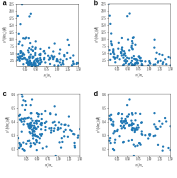
\includegraphics[width=0.99\linewidth]{img/SI-gpaw-alpha-emass.pdf}
  \caption{Relation between 2D polarizabilities and the effective
    carrier mass from Ref.\cite{Haastrup_2018}. 
    \textbf{a}. $\alpha_{\mathrm{2D}}^{\parallel}$ as a function of the
    electron mass $m_{e}^{*}$.  \textbf{b}. $\alpha_{\mathrm{2D}}^{\parallel}$ as a
    function of the hole mass
    $m_{h}^{*}$. \textbf{c}. $\alpha_{\mathrm{2D}}^{\perp}$ as a function of the
    electron mass $m_{e}^{*}$.  \textbf{d}. $\alpha_{\mathrm{2D}}^{\perp}$ as a
    function of the hole mass $m_{h}^{*}$. No apparent correlation
    between the 2D polarizabilities and the effective carrier masses
    is observed.}
  \label{fig:gpaw-2D-quantities-1}
\end{figure}

\begin{figure}[htbp]
  \centering
  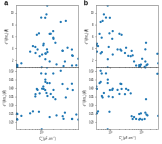
\includegraphics[width=0.95\linewidth]{img/SI-quantum-capacitance.pdf}
  \caption{Relation between the 2D polarizabilities with the quantum
    capacitance. \textbf{a} $\alpha_{\mathrm{2D}}^{\parallel}$ (top) and
    $\alpha_{\mathrm{2D}}^{\perp}$ (bottom) as functions of the quantum capacitance
    of the conduction band edge,
    $C_{\mathrm{Q}}^{\mathrm{C}}$. \textbf{b} $\alpha_{\mathrm{2D}}^{\parallel}$
    (top) and $\alpha_{\mathrm{2D}}^{\perp}$ (bottom) as functions of the quantum
    capacitance of the valence band edge,
    $C_{\mathrm{Q}}^{\mathrm{V}}$. Similar to the case of effective
    carrier mass, no apparent correlation between 2D polarizabilities
    and the quantum capacitance can be found.}
  \label{fig:gpaw-2D-quantities-2}
\end{figure}

\begin{figure}[htbp]
  \centering
  
\includegraphics[width=1.07\linewidth]{img/SI-gpaw-alpha-atomic-polarizability.pdf}
  \caption{Relation between the 2D polarizabilities
    (\textbf{a}. $\alpha_{\mathrm{2D}}^{\parallel}$ and
    \textbf{b}. $\alpha_{\mathrm{2D}}^{\perp}$) with the total atomic polarizability per area.}
  \label{fig:gpaw-2D-quantities-3}
\end{figure}

The quantum capacitance
$C_{\mathrm{Q}}(E)$ at certain energy level $E$ is calculated using
the relation $C_{\mathrm{Q}}(E)=\mathrm{DOS}(E)e^{2}$, where
$\mathrm{DOS}(E)$ is the density of states at the conduction or valence band edge (averaged by cell
area). The DOS value is calculated at the energy level with a charge
cutoff such that
$|n_{\mathrm{2D}}(E)| = 5 \times 10^{13}\ \mathrm{cm}^{-2}$, calculated by
the relation of accumulated charge $n_{\mathrm{2D}}(E)$ at CB or VB:
\begin{equation}
  \label{eq:CQ-method}
  |n_{\mathrm{2D}}(E)| = \left|\int_{E_{\mathrm{BE}}}^{E} \mathrm{DOS}(E') dE' \right|
\end{equation}
where $E_{\mathrm{BE}}$ is the energy of the CB or VB band edge.

The total polarizability $\alpha_{\mathrm{2D}}^{\mathrm{sum}}$ is calculated by the
summation of the atomic polarizabilities $\alpha_{\mathrm{2D}}^{\mathrm{atom}}$
\cite{Gould_2016_jctc} of individual atoms per area $A$, such that:
\begin{equation}
  \label{eq:atom-polar}
  \alpha_{\mathrm{2D}}^{\mathrm{sum}} = \frac{\sum_{i} \alpha^{\mathrm{atom}}_{i}}{A}
\end{equation}

From Figures \ref{fig:gpaw-2D-quantities-1} to
\ref{fig:gpaw-2D-quantities-3} we can see that none of the above
quantities have apparent relation with the 2D polarizabilities, as
compared with the bandgap and covalent thickness proposed in the main
text. 

%%%%%% pasted in 12/05/2018
\section{More discussion about the relation between 2D and 3D properties}
\label{sec:2D-3D}

\subsection{Comparing 2D and 3D Moss relations}
\label{ssec:theory-2D}
%\label{ssec:theory-2}
The 2D Moss-like relation $\alpha^{\parallel} \propto E_{g}^{-1}$ is
similar to the 3D Moss relation $\varepsilon \propto E_{g}^{-1/2}$,
with a different power law. Such difference in the power law can
indeed be explained by modern theory of dielectric properties. From
the 2D material to a bulk covalent semiconductor, the wave function
becomes periodic in all directions. Considering only one pair of
valence-conduction transition and uniform effective mass $m^{*}$,
extending the approach Eq. \ref{eq:alpha_perp_RPA} to the bulk
material, and using the Bloch presentation for wave functions in all
dimensions, we get \cite{Jiang_2017_Eg_Eb}:
\begin{equation}
  \begin{aligned}
    \label{eq:eps-bulk}
    \varepsilon_{\mathrm{bulk}} - 1 &\propto \int d^{3}\mathbf{k}
    {\displaystyle \frac{1}{(E_{\mathrm{g}} + {\displaystyle
          \frac{\hbar^{2} k^{2}}{m^{*}}})^{2}}}\\
    &= \int_{0}^{k_{\mathrm{BZ}}} {\displaystyle
      \frac{4 \pi k^{2}}{(E_{\mathrm{g}} + {\displaystyle \frac{\hbar^{2}
            k^{2}}{m^{*}}})^{2}}} dk
  \end{aligned}
\end{equation}
where $k_{\mathrm{BZ}}$ is the boundary for the Brillouin Zone. The
last step in Eq. \ref{eq:eps-bulk} assumes the integral within the
Brillouin Zone is equivalent to integral inside a sphere of
k-space. Let $\hbar^{2}/(2 m^{*})=\beta$, the integral becomes:
\begin{equation}
  \begin{aligned}
    \label{eq:integral-BZ-bulk}
    \varepsilon_{\mathrm{Bulk}} &\propto {\displaystyle \frac{2 \pi
        \mathrm{arctan}(\sqrt{\beta k^{2}/E_{\mathrm{g}}})}{\sqrt{E_{\mathrm{g}} \beta^{3}}}
        - \frac{2\pi k}{\beta(\beta +E_{\mathrm{g}}k^{2})}
      } \bigg\rvert_{0}^{k_{\mathrm{BZ}}}\\
      &\propto 1/\sqrt{E_{\mathrm{g}}}
  \end{aligned}
\end{equation}
when $\varepsilon_{\mathrm{Bulk}} \gg 1$. since generally
$\hbar^{2}k_{\mathrm{BZ}}^{2}/(2m^{*}) \gg
E_{\mathrm{g}}$ \cite{Finkenrath_1988}. The final result $\varepsilon_{\mathrm{Bulk}} \propto E_{\mathrm{g}}^{-1/2}$ recovers the original Moss relation for bulk semiconductors.


\subsection{Static 2D polarizability and 2D plasma frequency}
\label{ssec:omega-p}

A common approach for describing the bulk dielectric function of bulk
semiconductors is via the Lorentz oscillator model, where the
dielectric function is dominated by the plasma frequencies
$\omega_{\mathrm{3D}}^{\mathrm{p}}$ and bandgap $E_{\mathrm{g}}$ of
individual oscillators \cite{ketterson_physics_2016}. At zero optical
frequency and the static limit, the dielectric constant for single
oscillator is:
\begin{equation}
  \label{eq:eps-plas-3D}
  \varepsilon_{\mathrm{3D}} = 1 +
  \frac{\hbar^{2} (\omega_{\mathrm{3D}}^{\mathrm{p}})^{2}}{E_{\mathrm{g}}^{2}}
\end{equation}
where
$\omega_{\mathrm{3D}}^{\mathrm{p}} = {\displaystyle \sqrt{\frac{e^{2}
      n_{\mathrm{3D}}}{\varepsilon_{0} m_{e}}}}$, where
$n_{\mathrm{3D}}$ is the 3D number density of valence
electrons. Combine Eq. \ref{eq:eps-plas-3D} with 
Eq. \ref{main-eq:alpha-para-def}, we get:
\begin{equation}
  \begin{aligned}
  \label{eq:alpha-plas}
  \alpha_{\mathrm{2D}}^{\parallel} &= \frac{e^{2} n_{\mathrm{3D}} L}{m_{e} E_{\mathrm{g}}^{2}} \\
  &= \frac{e^{2} n_{\mathrm{2D}}}{m_{e} E_{\mathrm{g}}^{2}} \\
  &= \varepsilon_{0} \frac{\hbar^{2}
    (\omega_{\mathrm{2D}}^{\mathrm{p}})^{2}}{E_{\mathrm{g}}^{2}}
\end{aligned}
\end{equation}
where $n_{\mathrm{2D}} =n_{\mathrm{3D}} L$ is the 2D number density of
valence electrons and
$\omega_{\mathrm{2D}}^{p}=\omega_{\mathrm{3D}}^{p}\sqrt{L}$ is the 2D
plasma frequency at static limit \cite{Nazarov_2015_2D_3D}, as
discussed in the main text. Apparently $n_{\mathrm{2D}}$ and
$\omega_{\mathrm{2D}}^{p}$ defines the superlattice-independent 2D
quantity $\alpha_{\mathrm{2D}}^{\parallel}$, while its 3D counterpart
$\varepsilon_{\mathrm{3D}}$ is dependent on $L$. By defining the 2D
valence charge density
$\sigma_{\mathrm{2D}}^{\mathrm{v}}=n_{\mathrm{2D}}e$, we have also
calculated $\alpha_{\mathrm{2D}}^{\parallel}$ as a function of
$\sigma_{\mathrm{2D}}^{\mathrm{v}}/E_{\mathrm{g}}^{2}$ using Ref.\cite{Haastrup_2018} database, as shown in Figure \ref{fig:plasma}.
\begin{figure}[htbp]
  \centering
  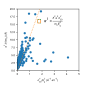
\includegraphics[width=0.85\linewidth]{img/SI-lorentz-model.pdf}
  \caption{Calculated $\alpha_{\mathrm{2D}}^{\parallel}$ as a function of
    $\sigma_{\mathrm{2D}}^{\mathrm{v}}/E_{\mathrm{g}}^{2}$ using data from Ref.\cite{Haastrup_2018}. The broken line shows the theoretical prediction
    from single-oscillator model.}
  \label{fig:plasma}
\end{figure}
It can be seen that, a large number of materials are close to the
theoretical value of
$\alpha_{\mathrm{2D}}^{\parallel} = \frac{e^{2} n_{\mathrm{3D}} L}{m_{e}
  E_{\mathrm{g}}^{2}}$ (broken line). However there are also many
violations to this simple relation, making such model not suitable for
quantitative prediction of the 2D dielectric nature, due to the
oversimplification of single Lorentz oscillator. Nevertheless, this
example shows excellently how the quantities in both dimensions are
related to each other.



\subsection{The relation between 2D and 3D physical quantities}
As schematically shown in Figure \ref{fig-2D-3D}, the physical
quantities related to the dielectric properties can be categorized
into (i) strictly 2D (microscopic), (ii) strictly 3D (macroscopic) and
(iii) valid both 2D and 3D.  $\alpha_{\mathrm{2D}}$ and $\varepsilon$ are the
starting point for the strictly 2D and 3D quantities, which require
distinct definitions when dimensionality changes. Such quantities
include (but not limited to):
\begin{enumerate}
\item The densities $n_{\mathrm{2D}}$ and $n_{\mathrm{3D}}$ for
  charge, polarization, electronic states, etc.
  
\item The plasma frequencies $\omega^{\mathrm{p}}_{\mathrm{2D}}$ and
  $\omega^{\mathrm{p}}_{\mathrm{2D}}$\cite{Nazarov_2015_2D_3D} (see
  Section \ref{ssec:omega-p} and Figure \ref{fig:plasma}).

\item The optical conductivity $\sigma_{\mathrm{2D}}$ and
  $\sigma_{\mathrm{3D}}$\cite{Bechstedt_2012,Matthes_2016}.
\end{enumerate}
These quantities have distinct units in both dimensions, and related
by $L$ (for density and optical conductivity) or $\sqrt{L}$ (for
plasma frequency), which requires prudent interpretation of
theoretical and experimental results. For instance, the experimentally
observed ``dielectric constant'' of monolayer 2D materials
\cite{Ning_2015,Li_2014,Yao_2014,Wu_2015} would be questionable
without considering the effect of mixed medium. Instead, the 2D slab
polarizability, either transformed from the vacuum-containing
macroscopic dielectric constant, or predicted from the bandgap and
geometry as proposed here, will be a better descriptor for the true 2D
dielectric nature. There are also
dimension-independent quantities that are valid for both 2D and 3D
systems, for instance the bandgap $E_{\mathrm{g}}$, exciton binding
energy $E_{\mathrm{b}}$, Bohr radius $r_{\mathrm{B}}$ of the exciton
as well as the Hamaker constant of van der Waals interaction
$A_{\mathrm{H}}$. All these quantities are well-defined and can be
measured in both dimensions, while their relation with the dielectric
property varies with dimensionality. The well-known examples are the
different Wannier-Mott laws for exciton binding energy
\cite{Olsen_2016_hydrogen}, the dielectric-bandgap relation
proposed here, and the distinct power laws for van der Waals
interactions \cite{Gobre_2013}. To get a accuracy description of
dielectric-related properties of the 2D materials and their
heterostructures, one has to distinguish between the 2D and 3D
properties, and choose a suitable relation with the
dimension-dependent and dimension-independent quantities.

\begin{figure}[htbp]
\centering
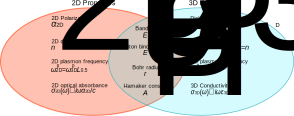
\includegraphics[width=0.85\linewidth]{img/fig-2D-vs-3D.pdf}
\caption{\label{fig-2D-3D} Dielectric-related physical quantities in
  both 2D (red circle) and 3D (cyan circle) systems. The
  dimension-dependent quantities can be related with $\alpha_{\mathrm{2D}}$ and
  $\varepsilon$, respectively. The intersection between the circles
  present the quantities are well-defined in both dimensions, but may have a
  different scaling relation with others quantities.}
\end{figure}


\section{More discussions about the dielectric anisotropy}
\label{sec:aniso}
\subsection{The 2D screening length}
\label{ssec:2D-screening}
Here we show a schematic drawing of the polarizability ellipsoid for a
2D material in Figure \ref{fig:ellipsoid}. As can be seen the
polarizability ellipsoid is ultraflat, with
$r_{0}^{\parallel} \gg r_{0}^{\perp}$, which is the origin of the high
dielectric anisotropy of 2D materials.

\begin{figure}[H]
  \centering
  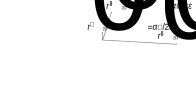
\includegraphics[width=0.9\linewidth]{img/SI-ellipsoid.pdf}
  \caption{Polarizability ellipsoid of a 2D material, the long axis
    equals $\alpha_{\mathrm{2D}}^{\parallel}/2\varepsilon_{0}$ and the short axis
    equals  $\alpha_{\mathrm{2D}}^{\perp}/2\varepsilon_{0}$}
  \label{fig:ellipsoid}
\end{figure}

\subsection{Choice of materials for Figure \ref{main-fig:aniso}}
\label{ssec:aniso-materials}
The dielectric anisotropy $\eta$ proposed in the main text is also
applied to other dimensions. Similar to the case of 2D and bulk
layered materials, $\epsilon$ is used to compare the anisotropy when
the material is periodic in all dimensions (bulk covalent materials),
while the polarizability $\alpha$ is used for reduced dimensional
materials.

The following types materials are chosen for comparison:
\begin{itemize}
\item Bulk covalent materials.  \\
  The list of materials and bandgap are chosen according to
  Ref. \citenum{sze_appendix_2006}, including IV-IV, III-V, II-VI, and
  IV-VI semiconductors. All these materials have isotropic dielectric
  properties.
\item Planar OSc \\
  The planar OScs include metal phthalocyanines, disk-like polycyclic
  aromatic hydrocarbon (PAHs), and benzene derivatives. The
  dimensionality of these materials are close to 2D materials due to
  their planar shape. The bandgap values (mostly at B3LYP density
  functional with 6-31G** basis sets) are extracted from the NIST
  Computational Chemistry Comparison and Benchmark Database
  (http://cccdb.nist.gov, Release 19, April 2018) and the
  polarizability values are obtained from
  Refs. \citenum{Miller_1990,Ramprasad_2006}.
\item Carbon nanotubes (CNT) \\
  Like 2D materials, CNTs are periodic along the 1D directions, and
  should be treated in a similar way to get the polarizability
  proportional to [Length]$^{2}$ \cite{Benedict_1995}. Semiconducting
  zigzag and armchair CNTs are considered, with their electronic
  properties obtained from Refs
  \citenum{Benedict_1995,Matsuda_2010}. and dielectric properties
  obtained from
  Refs. \citenum{Benedict_1995,Jensen_2000,Brothers_2008}.
\item Linear OSc \\
  We choose the linear polyacenes (linear PAHs from benzene to
  nonacene) and zigzag polyacetylene (1--9 repeating units) as model
  systems of linear OScs. The bandgaps are obtained from
  \citenum{Salzner_1998} and the polarizabilities are obtained from
  \citenum{Hinchliffe_2005}.
\item Fullerenes \\
  The bandgap of fullerenes (C$_{n}$ where $n=60*m^{2}$ where
  $m=1\sim{}7$) are taken from \citenum{Lin_1994} and the
  polarizabilities are taken from \citenum{Martin_2008}. All these
  materials have isotropic polarizability due to the high symmetry.
\end{itemize}

\subsection{Explanation for the separation between 2D and 3D regimes in Figure \ref{main-fig:aniso}}
\label{sssec:aniso-2}
In this section we give an analytical explanation for the separation
between the dielectric anisotropy indices of 2D and their bulk
counterparts. From Eqs. \ref{main-eq:alpha-para-def},
\ref{main-eq:alpha-perp-def} and \ref{main-eq:anisotropy},
$\eta_{\mathrm{Bulk}}$ of a bulk layered material is expressed as:
\begin{equation}
  \label{eq:eta-bulk}
  \begin{aligned}[t]
    \eta_{\mathrm{Bulk}} &= \frac{\varepsilon_{\mathrm{Bulk}}^{\perp}}
    {\varepsilon_{\mathrm{Bulk}}^{\parallel}}\\
    &= \frac{1}{\left(1 + {\displaystyle
          \frac{\alpha_{\mathrm{Bulk}}^{\parallel}}{\varepsilon_{0}L_{\mathrm{Bulk}}}}\right)
      \left(1 - {\displaystyle \frac{\alpha_{\mathrm{Bulk}}^{\perp}}{\varepsilon_{0}L_{\mathrm{Bulk}}}} \right)}\\
    &= \frac{1}{ \left[1-\left( {\displaystyle
            \frac{\alpha_{\mathrm{Bulk}}^{\perp}}{\alpha_{\mathrm{Bulk}}^{\parallel}}}\right)
        \left(
          {\displaystyle \frac{\alpha_{\mathrm{Bulk}}^{\parallel}}{\varepsilon_{0}
            L_{\mathrm{Bulk}}}} \right) \right]
      \left[ 1 + \left(
          {\displaystyle \frac{\alpha_{\mathrm{Bulk}}^{\parallel}}{\varepsilon_{0}
            L_{\mathrm{Bulk}}}} \right)\right]
    }
    % &= \frac{\left({\displaystyle \frac{\varepsilon_{0}L_{\mathrm{Bulk}}}{\alpha^{\parallel}_{\mathrm{Bulk}}}}\right)^{2}}
    % {\left({\displaystyle \frac{\varepsilon_{0}L_{\mathrm{Bulk}}}{\alpha_{\mathrm{Bulk}}^{\parallel}_{\mathrm{2D}}}}\right)^{2}    
      % -\left({\displaystyle \frac{\alpha_{\mathrm{Bulk}}^{\perp}}{\alpha_{\mathrm{Bulk}}^{\parallel}}}\right)
      % \left({\displaystyle \frac{\varepsilon_{0} L_{\mathrm{Bulk}}}{\alpha_{\mathrm{Bulk}}^{\parallel}}}\right)
      % + \left({\displaystyle \frac{\varepsilon_{0} L_{\mathrm{Bulk}}}{\alpha_{\mathrm{Bulk}}^{\parallel}}}\right)
      % -\left({\displaystyle \frac{\alpha_{\mathrm{Bulk}}^{\perp}}{\alpha_{\mathrm{Bulk}}^{\parallel}}}\right)}
  \end{aligned}
\end{equation}
Name take the fact that
$\alpha_{\mathrm{Bulk}}^{\parallel} \approx
\alpha^{\parallel}_{\mathrm{2D}}$ (Figure
\ref{main-fig-4}b), we name
$\alpha_{\mathrm{Bulk}}^{\parallel} /\epsilon_{0}L_{\mathrm{Bulk}}
\approx \alpha_{\mathrm{2D}}^{\parallel}/
\epsilon_{0}L_{\mathrm{Bulk}}$ as $\gamma$. Furthermore we name
$\alpha_{\mathrm{Bulk}}^{\perp}/\alpha_{\mathrm{Bulk}}^{\parallel}$ as
$\hat{\eta_{\mathrm{2D}}}$, that
$\hat{\eta}_{\mathrm{2D}} =
\alpha_{\mathrm{Bulk}}^{\perp}/\alpha_{\mathrm{Bulk}}^{\parallel} \geq
\alpha_{\mathrm{2D}}^{\perp}/\alpha_{\mathrm{2D}}^{\parallel}=\eta_{\mathrm{2D}}$,
and Eq. \ref{eq:eta-bulk} is reduced to:
\begin{equation}
  \label{eq:eta-bulk-2}
  \eta_{\mathrm{Bulk}} = \frac{1}{(1 - \hat{\eta}_{\mathrm{2D}} \gamma) (1 + \gamma)}
\end{equation}
The minimal value for $\eta_{\mathrm{Bulk}}$ when $\gamma>0$ is obtained by solving:
\begin{equation}
  \label{eq:eta-bulk-min}
  \frac{\partial \eta_{\mathrm{Bulk}}}{\partial \gamma}
  = \frac{2 \hat{\eta}_{\mathrm{2D}} \gamma + \hat{\eta}_{\mathrm{2D}} - 1}
  {(\gamma+1)^{2}(1 - \hat{\eta}_{\mathrm{2D}} \gamma)^{2}} = 0
\end{equation}
which gives that
$\eta_{\mathrm{Bulk}} \geq \frac{4
  \hat{\eta}_{\mathrm{2D}}}{(\hat{\eta}_{\mathrm{2D}} + 1)^{2}}$,
where the minimal value is taken at
$\gamma = \frac{1}{2}(\frac{1}{\hat{\eta}_{\mathrm{2D}}} - 1)$. Since
$\frac{4 \hat{\eta}_{\mathrm{2D}}}{(\hat{\eta}_{\mathrm{2D}} +
  1)^{2}}$ monotonically increases when
$0 < \hat{\eta}_{\mathrm{2D}} < 1$, we get the comparison between the
dielectric anisotropy indices between 2D materials and their bulk
counterparts:
\begin{equation}
  \label{eq:aniso-final}
\eta_{\mathrm{Bulk}} \geq \frac{4
  \eta_{\mathrm{2D}}}{(\eta_{\mathrm{2D}} + 1)^{2}} \geq
\eta_{\mathrm{2D}} 
\end{equation}
Since $\gamma$ is actually $2r_{0}^{\parallel}/L_{\mathrm{Bulk}}$, the
ratio between the in-plane screening length $r_{0}^{\parallel}$ and
inter-plane distance $L_{\mathrm{Bulk}}$, and in general
$r_{0}^{\parallel} \gg L_{\mathrm{Bulk}}$, we can conclude that the
case when $\eta_{\mathrm{Bulk}} = \eta_{\mathrm{2D}}$ only happens
when $\eta_{\mathrm{2D}}$ is much smaller than 1. Therefore the
separation between the 2D and 3D regimes in Figure
\ref{main-fig:aniso} is explained.




%%%%%%pasted!



\section{Raw data from first principles calculations}
\label{sec:raw}
\subsection{Quantities from first principles calculation}

Table S2 shows the parameters and results from the
first principles calculations for the 2D materials studied. The 2D
screening lengthes $r_{0}^{\parallel}$ and $r_{0}^{\perp}$ can be
obtained by multiplying $2 \pi$ to the columns
$\alpha_{\mathrm{2D}}^{\parallel}/(4\pi \varepsilon_{0})$ and
$\alpha_{\mathrm{2D}}^{\perp}/(4\pi \varepsilon_{0})$, respectively.

% \documentclass{article}
% \usepackage[margin=1in]{geometry}
% \usepackage{multirow, float}
% \usepackage{ltablex}
% \usepackage{amsmath}
% \begin{document}

\begin{center}
  \footnotesize
\setlongtables
\begin{tabularx}{1.1\linewidth}{lXXXXXXXXX}
      \caption{Raw data of the materials calculated in this study.}\\
    \hline
    Material & L (\AA) & HSE06 $E_{\mathrm{g}}^{\mathrm{min}}$ (eV) & PBE $E_{\mathrm{g}}^{\mathrm{min}}$ (eV) & PBE $E_{\mathrm{g}}^{\mathrm{direct}}$ (eV) & $\varepsilon_{\mathrm{SL}}^{\mathrm{xx}}$ & $\varepsilon_{\mathrm{SL}}^{\mathrm{yy}}$ & $\varepsilon_{\mathrm{SL}}^{\mathrm{zz}}$ & $\alpha_{\mathrm{2D}}^{\parallel}/(4\pi \varepsilon_{0})$ (\AA) & $\alpha_{\mathrm{2D}}^{\perp}/(4\pi \varepsilon_{0})$ (\AA)\\
    \hline
    \endhead
    1T-TiO$_{2}$ & 26.668  & 4.010  & 3.096  & 2.467  & 1.887  & 1.887  & 1.123  & 1.882  & 0.232 \\
    2H-TiO$_{2}$ & 27.648  & 2.520  & 1.808  & 1.103  & 1.852  & 1.852  & 1.133  & 1.875  & 0.258 \\
    1T-TiSe$_{2}$ & 33.049  & 1.360  & 1.372  & 0.505  & 3.029  & 3.029  & 1.190  & 5.336  & 0.420 \\
    1T-ZrO$_{2}$ & 26.561  & 6.320  & 5.039  & 4.431  & 1.569  & 1.569  & 1.117  & 1.203  & 0.221 \\
    1T-ZrS$_{2}$ & 32.622  & 2.010  & 1.643  & 1.180  & 2.329  & 2.329  & 1.159  & 3.450  & 0.356 \\
    1T-ZrSe$_{2}$ & 34.056  & 0.890  & 0.961  & 0.371  & 2.794  & 2.794  & 1.172  & 4.862  & 0.398 \\
    2H-ZrO$_{2}$ & 28.188  & 3.130  & 2.264  & 1.690  & 1.619  & 1.619  & 1.121  & 1.389  & 0.242 \\
    2H-ZrSe$_{2}$ & 33.692  & 1.500  & 1.382  & 0.738  & 2.448  & 2.448  & 1.190  & 3.882  & 0.428 \\
    2H-ZrTe$_{2}$ & 35.904  & 0.900  & 1.216  & 0.284  & 3.171  & 3.171  & 1.207  & 6.203  & 0.490 \\
    1T-HfO$_{2}$ & 26.636  & 6.580  & 5.471  & 4.830  & 1.521  & 1.521  & 1.117  & 1.104  & 0.222 \\
    1T-HfS$_{2}$ & 32.558  & 2.010  & 1.949  & 1.224  & 2.250  & 2.250  & 1.204  & 3.239  & 0.439 \\
    1T-HfSe$_{2}$ & 33.916  & 1.070  & 1.215  & 0.435  & 2.702  & 2.702  & 1.180  & 4.594  & 0.412 \\
    2H-HfO$_{2}$ & 28.167  & 3.400  & 2.552  & 1.948  & 1.555  & 1.555  & 1.124  & 1.244  & 0.247 \\
    2H-HfS$_{2}$ & 32.678  & 1.890  & 1.831  & 1.068  & 2.087  & 2.087  & 1.177  & 2.827  & 0.391 \\
    2H-HfSe$_{2}$ & 33.419  & 1.530  & 1.754  & 0.819  & 2.390  & 2.390  & 1.191  & 3.697  & 0.426 \\
    2H-HfTe$_{2}$ & 35.629  & 0.700  & 1.251  & 0.121  & 3.072  & 3.072  & 1.208  & 5.875  & 0.488 \\
    1T-GeO$_{2}$ & 26.526  & 5.740  & 6.118  & 3.466  & 1.453  & 1.453  & 1.115  & 0.956  & 0.218 \\
    1T-GeS$_{2}$ & 31.883  & 1.580  & 2.697  & 0.726  & 2.302  & 2.302  & 1.169  & 3.303  & 0.367 \\
    1T-GeO$_{2}$ & 27.908  & 2.990  & 4.643  & 1.335  & 1.570  & 1.570  & 1.127  & 1.266  & 0.250 \\
    1T-SnO$_{2}$ & 27.147  & 4.570  & 5.840  & 2.649  & 1.449  & 1.449  & 1.114  & 0.970  & 0.221 \\
    1T-SnS$_{2}$ & 32.793  & 2.530  & 2.859  & 1.574  & 2.059  & 2.059  & 1.166  & 2.764  & 0.372 \\
    1T-SnSe$_{2}$ & 34.077  & 1.490  & 1.466  & 0.751  & 2.437  & 2.437  & 1.169  & 3.897  & 0.392 \\
    2H-SnO$_{2}$ & 28.938  & 1.960  & 4.661  & 0.647  & 1.590  & 1.590  & 1.124  & 1.359  & 0.254 \\
    2H-SnS$_{2}$ & 32.873  & 1.590  & 1.072  & 0.750  & 2.164  & 2.164  & 1.180  & 3.045  & 0.399 \\
    1T-PbO$_{2}$ & 27.862  & 2.600  & 3.578  & 1.330  & 1.709  & 1.709  & 1.121  & 1.572  & 0.239 \\
    BN & 29.995  & 5.640  & 5.688  & 5.592  & 1.366  & 1.366  & 1.072  & 0.874  & 0.160 \\
    C$_{2}$F$_{2}$ & 31.998  & 5.000  & 3.173  & 3.173  & 1.318  & 1.348  & 1.123  & 0.810  & 0.279 \\
    P$_{4}$ & 27.097  & 1.600  & 0.888  & 0.895  & 2.894  & 3.115  & 1.196  & 4.084  & 0.353 \\
    C$_{2}$H$_{2}$ & 31.015  & 4.360  & 3.468  & 3.468  & 1.288  & 1.288  & 1.094  & 0.711  & 0.212\\ 
    1T-NiO$_{2}$ & 26.112  & 3.170  & 1.828  & 1.198  & 2.763  & 2.763  & 1.129  & 3.663  & 0.237\\ 
    1T-PdO$_{2}$ & 26.712  & 3.210  & 2.475  & 1.397  & 2.368  & 2.368  & 1.116  & 2.908  & 0.221 \\
    1T-PdS$_{2}$ & 30.361  & 1.800  & 2.487  & 1.178  & 3.888  & 3.888  & 1.169  & 6.978  & 0.349 \\
    1T-PtO$_{2}$ & 26.316  & 3.540  & 2.602  & 1.691  & 2.114  & 2.114  & 1.116  & 2.333  & 0.218 \\
    1T-PtS$_{2}$ & 30.239  & 2.700  & 2.022  & 1.714  & 3.086  & 3.086  & 1.163  & 5.020  & 0.337 \\
    1T-PdSe$_{2}$ & 31.080  & 0.970  & 1.917  & 0.534  & 4.958  & 4.958  & 1.178  & 9.789  & 0.374 \\
    1T-NiS$_{2}$ & 29.616  & 0.980  & 1.797  & 0.523  & 4.691  & 4.691  & 1.173  & 8.699  & 0.348 \\
    1T-PtSe$_{2}$ & 31.058  & 1.210  & 2.710  & 1.180  & 3.643  & 3.643  & 1.175  & 6.532  & 0.368 \\
    Ga$_{2}$Se$_{2}$ & 30.000  & 2.810  & 2.657  & 1.764  & 2.640  & 2.640  & 1.281  & 3.915  & 0.524 \\
    Ga$_{2}$S$_{2}$ & 30.000  & 3.250  & 3.351  & 2.358  & 2.329  & 2.329  & 1.256  & 3.173  & 0.487 \\
    CdCl$_{2}$ & 31.085 & 5.18 & 3.78 & 3.78 & 1.48 & 1.48 & 1.157 & 1.187 & 0.336 \\
    CdI$_{2}$ & 35.281  & 3.150  & 1.706  & 1.528  & 1.804  & 1.804  & 1.192  & 2.257  & 0.452 \\
    2H-MoS$_{2}$ & 32.296  & 2.240  & 1.594  & 1.594  & 3.475  & 3.475  & 1.183  & 6.361  & 0.398 \\
    2H-MoSe$_{2}$ & 40.854 & 1.83 & 1.38 &   1.38 & 3.231 &  3.231 & 1.154 & 7.253 & 0.433 \\
    2H-WS$_{2}$ & 32.271  & 2.280  & 1.540  & 1.540  & 3.214  & 3.214  & 1.180  & 5.686  & 0.392 \\
    2H-WSe$_{2}$ & 32.965  & 1.930  & 1.253  & 1.253  & 3.485  & 3.485  & 1.197  & 6.519  & 0.432 \\
    2H-WO$_{2}$ & 29.183  & 2.000  & 1.693  & 1.359  & 2.519  & 2.519  & 1.123  & 3.528  & 0.254 \\
    2H-MoO$_{2}$ & 29.231  & 1.560  & 1.648  & 0.952  & 2.918  & 2.918  & 1.129  & 4.462  & 0.266 \\
    2H-MoTe$_{2}$ & 34.061  & 1.440  & 0.946  & 0.946  & 4.412  & 4.412  & 1.220  & 9.248  & 0.489 \\
    2H-WTe$_{2}$ & 33.883  & 1.300  & 0.731  & 0.731  & 4.158  & 4.158  & 1.230  & 8.515  & 0.504 \\
    2H-CrS$_{2}$ & 31.759  & 1.400  & 0.902  & 0.902  & 4.647  & 4.647  & 1.183  & 9.217  & 0.391 \\
    2H-CrSe$_{2}$ & 32.446  & 1.150  & 0.704  & 0.704  & 5.364  & 5.364  & 1.201  & 11.268  & 0.432 \\
    2H-CrO$_{2}$ & 28.027  & 0.990  & 1.596  & 0.424  & 3.961  & 3.961  & 1.134  & 6.604  & 0.264 \\
    2H-CrTe$_{2}$ & 33.684 & 0.870 & 0.450 & 0.450 & 1.728 & 1.728 & 1.167 & 1.951 & 0.384 \\
    2H-TiS$_{2}$ & 32.199  & 1.610  & 1.284  & 0.692  & 2.634  & 2.634  & 1.184  & 4.187  & 0.398 \\
    1T-PtTe$_{2}$ & 32.005  & 0.490  & 1.809  & 0.366  & 4.726  & 4.726  & 1.200  & 9.490  & 0.424 \\
    MAPbBr$_{3}$ & 23.018 & 2.95 & 2.06 & 2.06 & 1.608 & 1.778 & 1.527 & 1.265 & 0.632 \\
    \hline
  \end{tabularx}

\end{center}
% \end{document}


\subsection{Density of States (DOS) plots for the materials studied}
\label{sec:DOS}


\begin{center}
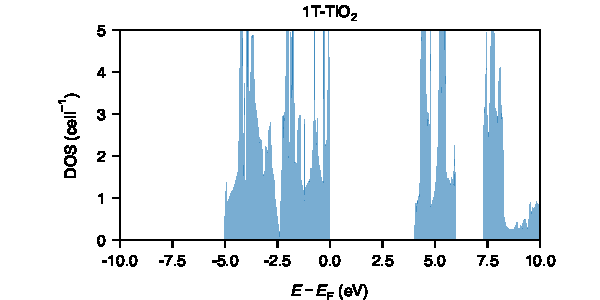
\includegraphics[width=.9\linewidth]{img/SI_figs/1T-TiO2-DOS.pdf}
\end{center}
\begin{center}
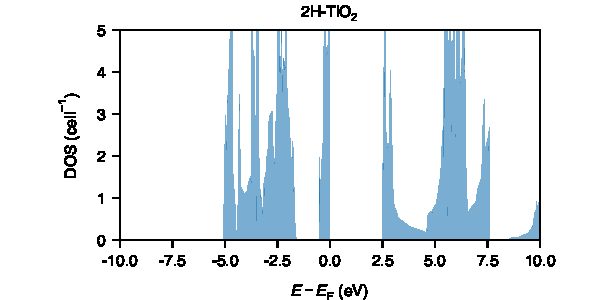
\includegraphics[width=.9\linewidth]{img/SI_figs/2H-TiO2-DOS.pdf}
\end{center}
\begin{center}
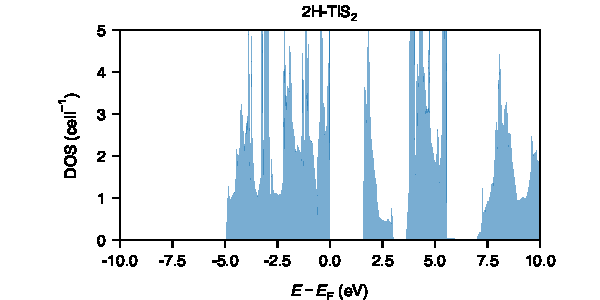
\includegraphics[width=.9\linewidth]{img/SI_figs/2H-TiS2-DOS.pdf}
\end{center}
\begin{center}
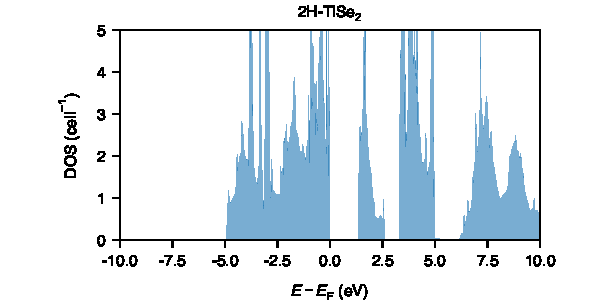
\includegraphics[width=.9\linewidth]{img/SI_figs/2H-TiSe2-DOS.pdf}
\end{center}
\begin{center}
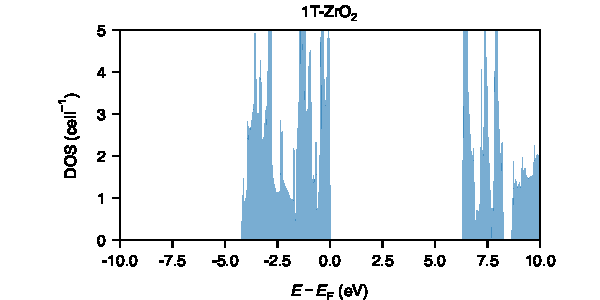
\includegraphics[width=.9\linewidth]{img/SI_figs/1T-ZrO2-DOS.pdf}
\end{center}
\begin{center}
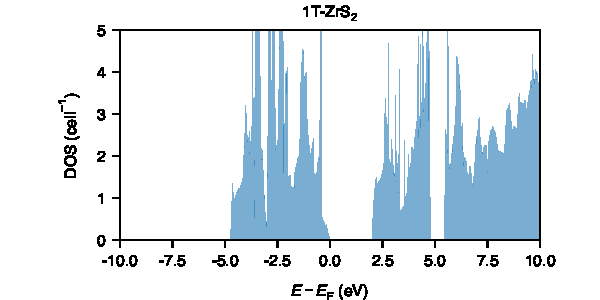
\includegraphics[width=.9\linewidth]{img/SI_figs/1T-ZrS2-DOS.pdf}
\end{center}
\begin{center}
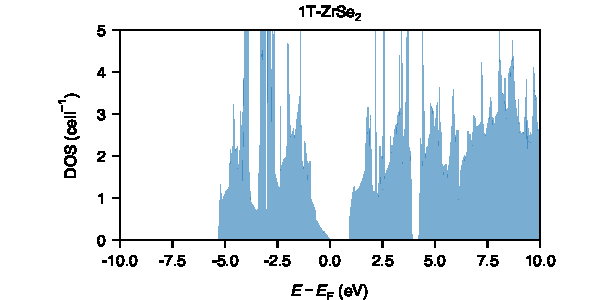
\includegraphics[width=.9\linewidth]{img/SI_figs/1T-ZrSe2-DOS.pdf}
\end{center}
\begin{center}
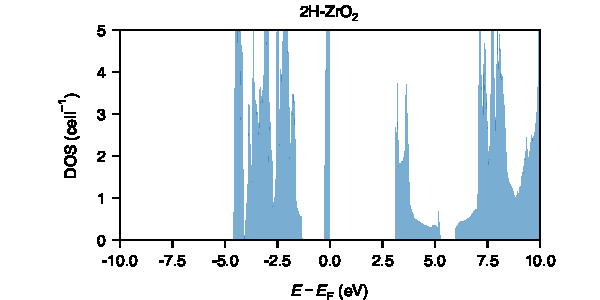
\includegraphics[width=.9\linewidth]{img/SI_figs/2H-ZrO2-DOS.pdf}
\end{center}
\begin{center}
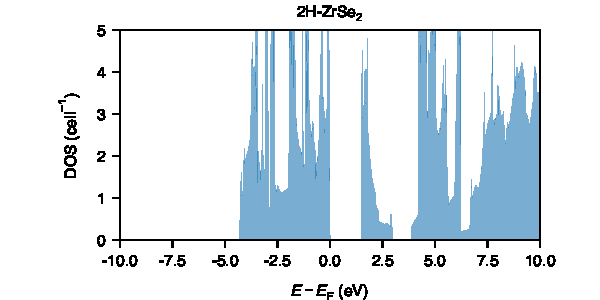
\includegraphics[width=.9\linewidth]{img/SI_figs/2H-ZrSe2-DOS.pdf}
\end{center}
\begin{center}
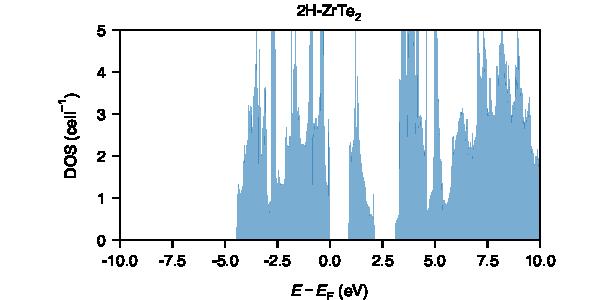
\includegraphics[width=.9\linewidth]{img/SI_figs/2H-ZrTe2-DOS.pdf}
\end{center}
\begin{center}
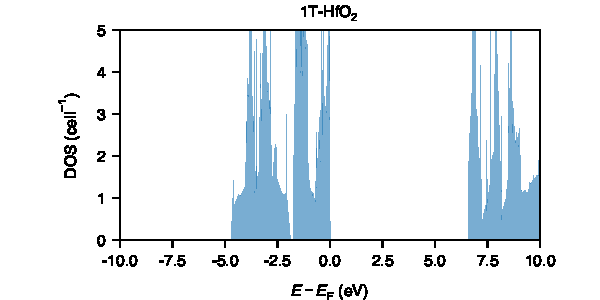
\includegraphics[width=.9\linewidth]{img/SI_figs/1T-HfO2-DOS.pdf}
\end{center}
\begin{center}
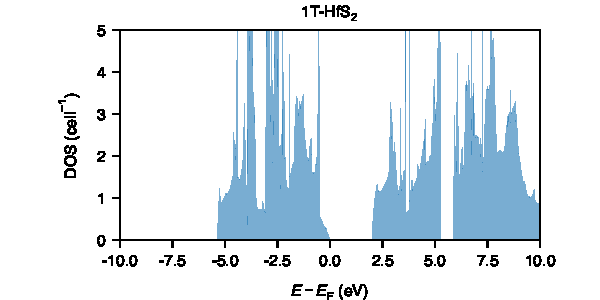
\includegraphics[width=.9\linewidth]{img/SI_figs/1T-HfS2-DOS.pdf}
\end{center}
\begin{center}
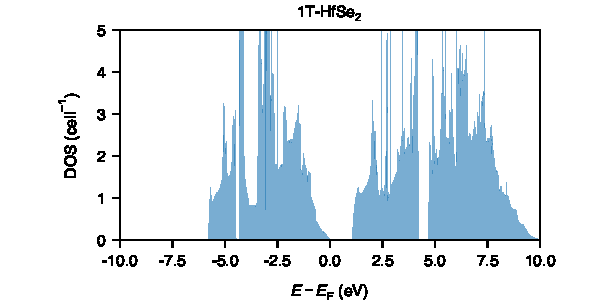
\includegraphics[width=.9\linewidth]{img/SI_figs/1T-HfSe2-DOS.pdf}
\end{center}
\begin{center}
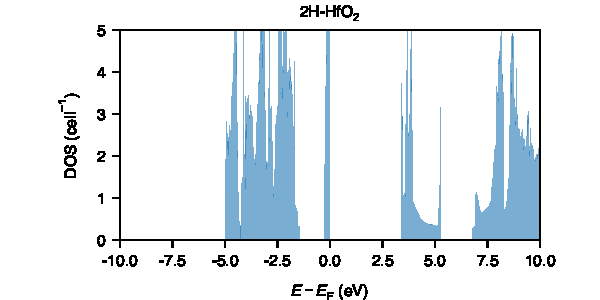
\includegraphics[width=.9\linewidth]{img/SI_figs/2H-HfO2-DOS.pdf}
\end{center}
\begin{center}
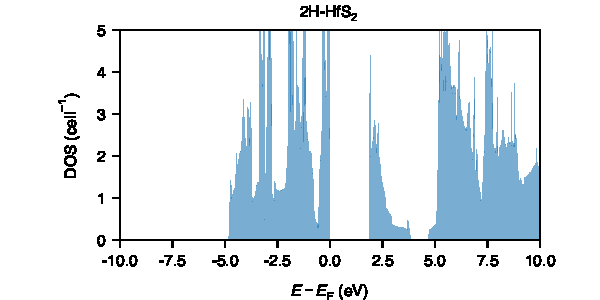
\includegraphics[width=.9\linewidth]{img/SI_figs/2H-HfS2-DOS.pdf}
\end{center}
\begin{center}
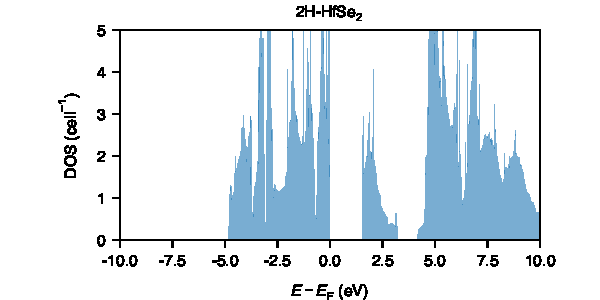
\includegraphics[width=.9\linewidth]{img/SI_figs/2H-HfSe2-DOS.pdf}
\end{center}
\begin{center}
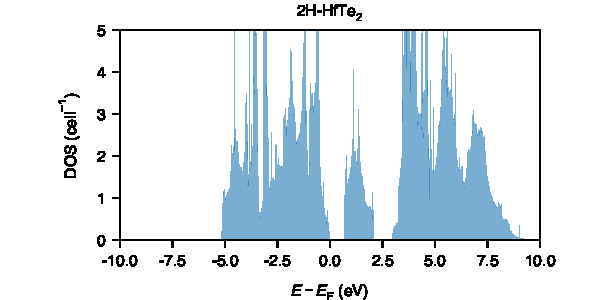
\includegraphics[width=.9\linewidth]{img/SI_figs/2H-HfTe2-DOS.pdf}
\end{center}
\begin{center}
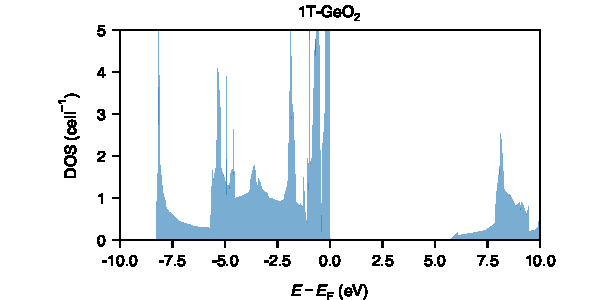
\includegraphics[width=.9\linewidth]{img/SI_figs/1T-GeO2-DOS.pdf}
\end{center}
\begin{center}
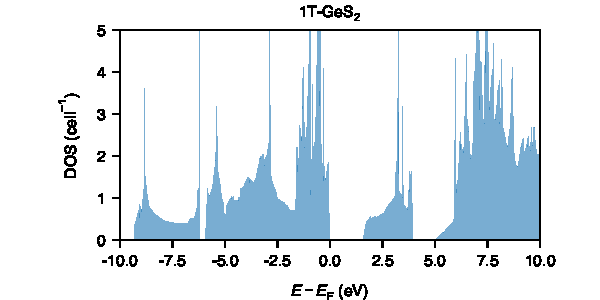
\includegraphics[width=.9\linewidth]{img/SI_figs/1T-GeS2-DOS.pdf}
\end{center}
\begin{center}
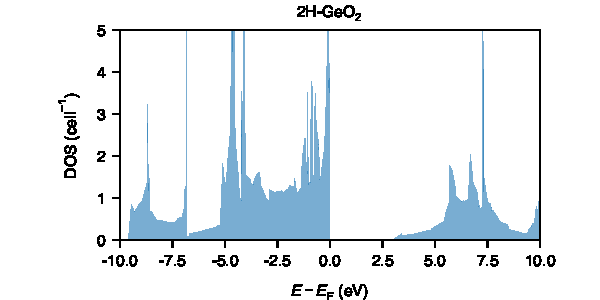
\includegraphics[width=.9\linewidth]{img/SI_figs/2H-GeO2-DOS.pdf}
\end{center}
\begin{center}
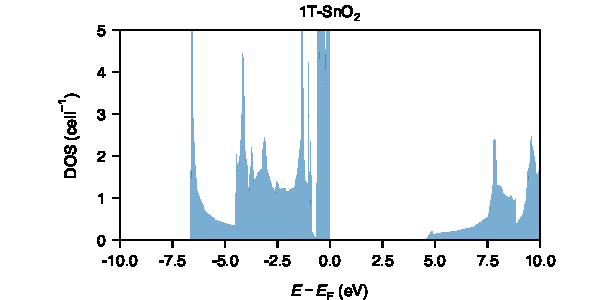
\includegraphics[width=.9\linewidth]{img/SI_figs/1T-SnO2-DOS.pdf}
\end{center}
\begin{center}
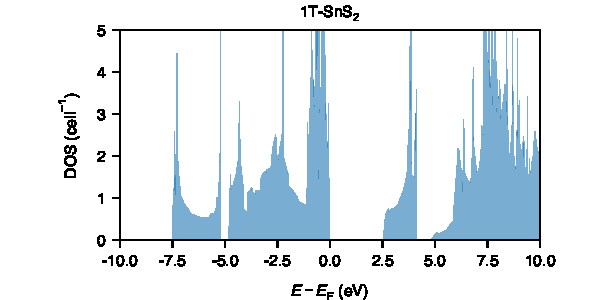
\includegraphics[width=.9\linewidth]{img/SI_figs/1T-SnS2-DOS.pdf}
\end{center}
\begin{center}
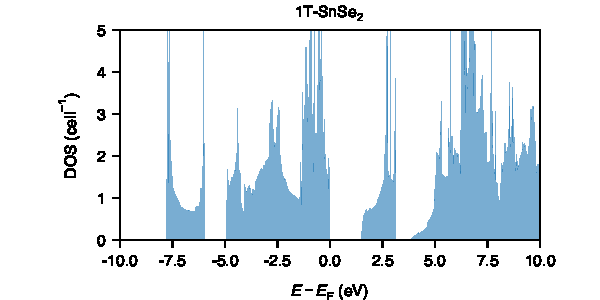
\includegraphics[width=.9\linewidth]{img/SI_figs/1T-SnSe2-DOS.pdf}
\end{center}
\begin{center}
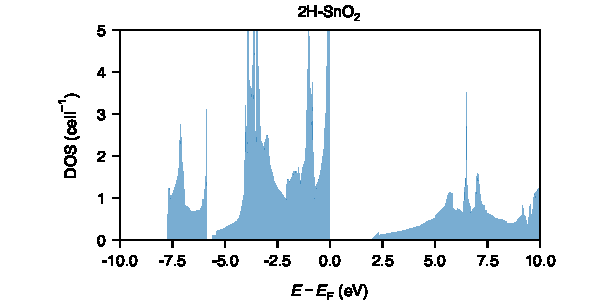
\includegraphics[width=.9\linewidth]{img/SI_figs/2H-SnO2-DOS.pdf}
\end{center}
\begin{center}
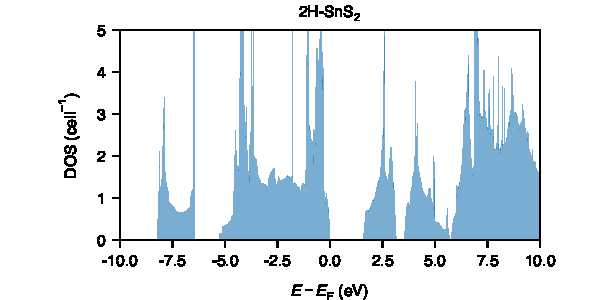
\includegraphics[width=.9\linewidth]{img/SI_figs/2H-SnS2-DOS.pdf}
\end{center}
\begin{center}
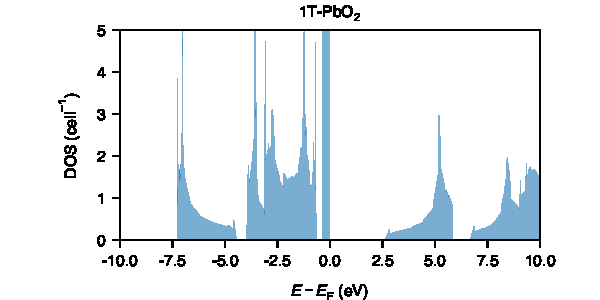
\includegraphics[width=.9\linewidth]{img/SI_figs/1T-PbO2-DOS.pdf}
\end{center}
\begin{center}
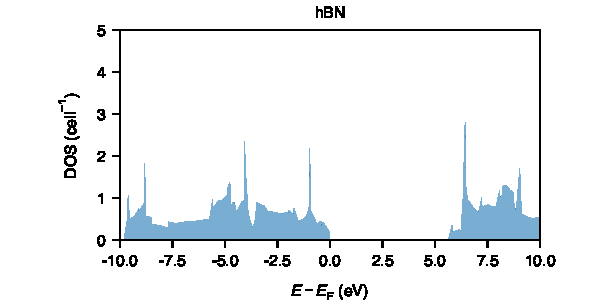
\includegraphics[width=.9\linewidth]{img/SI_figs/hBN-DOS.pdf}
\end{center}
\begin{center}
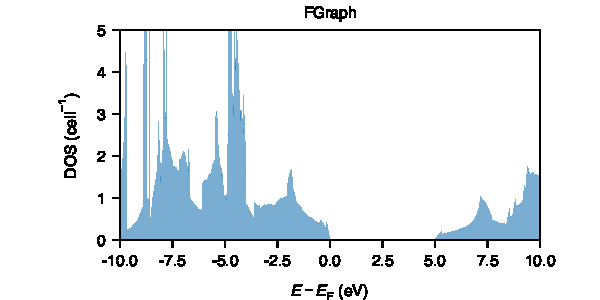
\includegraphics[width=.9\linewidth]{img/SI_figs/FGraph-DOS.pdf}
\end{center}
\begin{center}
\includegraphics[width=.9\linewidth]{img/SI_figs/Phosphorene-DOS.pdf}
\end{center}
\begin{center}
\includegraphics[width=.9\linewidth]{img/SI_figs/Graphane-DOS.pdf}
\end{center}
\begin{center}
\includegraphics[width=.9\linewidth]{img/SI_figs/1T-NiO2-DOS.pdf}
\end{center}
\begin{center}
\includegraphics[width=.9\linewidth]{img/SI_figs/1T-PdO2-DOS.pdf}
\end{center}
\begin{center}
\includegraphics[width=.9\linewidth]{img/SI_figs/1T-PdS2-DOS.pdf}
\end{center}
\begin{center}
\includegraphics[width=.9\linewidth]{img/SI_figs/1T-PtO2-DOS.pdf}
\end{center}
\begin{center}
\includegraphics[width=.9\linewidth]{img/SI_figs/1T-PtS2-DOS.pdf}
\end{center}
\begin{center}
\includegraphics[width=.9\linewidth]{img/SI_figs/1T-PdSe2-DOS.pdf}
\end{center}
\begin{center}
\includegraphics[width=.9\linewidth]{img/SI_figs/1T-NiS2-DOS.pdf}
\end{center}
\begin{center}
\includegraphics[width=.9\linewidth]{img/SI_figs/1T-PtSe2-DOS.pdf}
\end{center}
\begin{center}
\includegraphics[width=.9\linewidth]{img/SI_figs/GaSe-DOS.pdf}
\end{center}
\begin{center}
\includegraphics[width=.9\linewidth]{img/SI_figs/GaS-DOS.pdf}
\end{center}
\begin{center}
\includegraphics[width=.9\linewidth]{img/SI_figs/CdI2-DOS.pdf}
\end{center}
\begin{center}
\includegraphics[width=.9\linewidth]{img/SI_figs/2H-MoS2-DOS.pdf}
\end{center}
\begin{center}
\includegraphics[width=.9\linewidth]{img/SI_figs/2H-WS2-DOS.pdf}
\end{center}
\begin{center}
\includegraphics[width=.9\linewidth]{img/SI_figs/2H-WSe2-DOS.pdf}
\end{center}
\begin{center}
\includegraphics[width=.9\linewidth]{img/SI_figs/2H-WO2-DOS.pdf}
\end{center}
\begin{center}
\includegraphics[width=.9\linewidth]{img/SI_figs/2H-MoO2-DOS.pdf}
\end{center}
\begin{center}
\includegraphics[width=.9\linewidth]{img/SI_figs/2H-MoTe2-DOS.pdf}
\end{center}
\begin{center}
\includegraphics[width=.9\linewidth]{img/SI_figs/2H-WTe2-DOS.pdf}
\end{center}
\begin{center}
\includegraphics[width=.9\linewidth]{img/SI_figs/2H-CrS2-DOS.pdf}
\end{center}
\begin{center}
\includegraphics[width=.9\linewidth]{img/SI_figs/2H-CrSe2-DOS.pdf}
\end{center}
\begin{center}
\includegraphics[width=.9\linewidth]{img/SI_figs/2H-CrO2-DOS.pdf}
\end{center}

\subsection{Band structures of 2D materials calculated}
\label{sec:bs}

% \documentclass{article}

% \usepackage{graphicx}
% \usepackage{float}

% \begin{document}
\maxdeadcycles=200
\begin{figure}[htbp]
  \centering
  {\bfseries \sffamily 1T-TiO$_{2}$}\\
  % \vskip -2cm
  \includegraphics[width=0.45\linewidth, angle=-90, trim={3cm, 0cm, 2cm, 0cm}, clip]{img/SI_figs/BS/1T-TiO2.eps}
\end{figure}

\begin{figure}[htbp]
  \centering
  {\bfseries \sffamily 2H-TiO$_{2}$}\\
  % \vskip -2cm
  \includegraphics[width=0.45\linewidth, angle=-90, trim={3cm, 0cm, 2cm, 0cm}, clip]{img/SI_figs/BS/2H-TiO2.eps}
\end{figure}

\begin{figure}[htbp]
  \centering
  {\bfseries \sffamily 2H-TiS$_{2}$}\\
  % \vskip -2cm
  \includegraphics[width=0.45\linewidth, angle=-90, trim={3cm, 0cm, 2cm, 0cm}, clip]{img/SI_figs/BS/2H-TiS2.eps}
\end{figure}

\begin{figure}[htbp]
  \centering
  {\bfseries \sffamily 2H-TiSe$_{2}$}\\
  % \vskip -2cm
  \includegraphics[width=0.45\linewidth, angle=-90, trim={3cm, 0cm, 2cm, 0cm}, clip]{img/SI_figs/BS/2H-TiSe2.eps}
\end{figure}

\begin{figure}[htbp]
  \centering
  {\bfseries \sffamily 1T-ZrO$_{2}$}\\
\includegraphics[width=0.45\linewidth, angle=-90, trim={2.9cm, 0cm, 2cm, 0cm}, clip]{img/SI_figs/BS/1T-ZrO2.eps}
\end{figure}

\begin{figure}[htbp]
\centering
{\bfseries \sffamily 1T-ZrS$_{2}$}\\
\includegraphics[width=0.45\linewidth, angle=-90, trim={2.9cm, 0cm, 2cm, 0cm}, clip]{img/SI_figs/BS/1T-ZrS2.eps}
\end{figure}

\begin{figure}[htbp]
\centering
{\bfseries \sffamily 1T-ZrSe$_{2}$}\\
\includegraphics[width=0.45\linewidth, angle=-90, trim={2.9cm, 0cm, 2cm, 0cm}, clip]{img/SI_figs/BS/1T-ZrSe2.eps}
\end{figure}

\begin{figure}[htbp]
\centering
{\bfseries \sffamily 2H-ZrO$_{2}$}\\
\includegraphics[width=0.45\linewidth, angle=-90, trim={2.9cm, 0cm, 2cm, 0cm}, clip]{img/SI_figs/BS/2H-ZrO2.eps}
\end{figure}

\begin{figure}[htbp]
\centering
{\bfseries \sffamily 2H-ZrSe$_{2}$}\\
\includegraphics[width=0.45\linewidth, angle=-90, trim={2.9cm, 0cm, 2cm, 0cm}, clip]{img/SI_figs/BS/2H-ZrSe2.eps}
\end{figure}

\begin{figure}[htbp]
\centering
{\bfseries \sffamily 2H-ZrTe$_{2}$}\\
\includegraphics[width=0.45\linewidth, angle=-90, trim={2.9cm, 0cm, 2cm, 0cm}, clip]{img/SI_figs/BS/2H-ZrTe2.eps}
\end{figure}

\begin{figure}[htbp]
\centering
{\bfseries \sffamily 1T-HfO$_{2}$}\\
\includegraphics[width=0.45\linewidth, angle=-90, trim={2.9cm, 0cm, 2cm, 0cm}, clip]{img/SI_figs/BS/1T-HfO2.eps}
\end{figure}

\begin{figure}[htbp]
\centering
{\bfseries \sffamily 1T-HfS$_{2}$}\\
\includegraphics[width=0.45\linewidth, angle=-90, trim={2.9cm, 0cm, 2cm, 0cm}, clip]{img/SI_figs/BS/1T-HfS2.eps}
\end{figure}

\begin{figure}[htbp]
\centering
{\bfseries \sffamily 1T-HfSe$_{2}$}\\
\includegraphics[width=0.45\linewidth, angle=-90, trim={2.9cm, 0cm, 2cm, 0cm}, clip]{img/SI_figs/BS/1T-HfSe2.eps}
\end{figure}

\begin{figure}[htbp]
\centering
{\bfseries \sffamily 2H-HfO4$_{2}$}\\
\includegraphics[width=0.45\linewidth, angle=-90, trim={2.9cm, 0cm, 2cm, 0cm}, clip]{img/SI_figs/BS/2H-HfO2.eps}
\end{figure}

% \begin{figure}[htbp]
% \centering
% {\bfseries \sffamily 2H-HfS$_{2}$}\\
% \includegraphics[width=0.45\linewidth, angle=-90, trim={2.9cm, 0cm, 2cm, 0cm}, clip]{img/SI_figs/BS/2H-HfS2.eps}
% \end{figure}

\begin{figure}[htbp]
\centering
{\bfseries \sffamily 2H-HfSe$_{2}$}\\
\includegraphics[width=0.45\linewidth, angle=-90, trim={2.9cm, 0cm, 2cm, 0cm}, clip]{img/SI_figs/BS/2H-HfSe2.eps}
\end{figure}

\begin{figure}[htbp]
\centering
{\bfseries \sffamily 2H-HfTe$_{2}$}\\
\includegraphics[width=0.45\linewidth, angle=-90, trim={2.9cm, 0cm, 2cm, 0cm}, clip]{img/SI_figs/BS/2H-HfTe2.eps}
\end{figure}

\begin{figure}[htbp]
\centering
{\bfseries \sffamily 1T-GeO$_{2}$}\\
\includegraphics[width=0.45\linewidth, angle=-90, trim={2.9cm, 0cm, 2cm, 0cm}, clip]{img/SI_figs/BS/1T-GeO2.eps}
\end{figure}

\begin{figure}[htbp]
\centering
{\bfseries \sffamily 1T-GeS$_{2}$}\\
\includegraphics[width=0.45\linewidth, angle=-90, trim={2.9cm, 0cm, 2cm, 0cm}, clip]{img/SI_figs/BS/1T-GeS2.eps}
\end{figure}

\begin{figure}[htbp]
\centering
{\bfseries \sffamily 2H-GeO$_{2}$}\\
\includegraphics[width=0.45\linewidth, angle=-90, trim={2.9cm, 0cm, 2cm, 0cm}, clip]{img/SI_figs/BS/2H-GeO2.eps}
\end{figure}

\begin{figure}[htbp]
\centering
{\bfseries \sffamily 1T-SnO$_{2}$}\\
\includegraphics[width=0.45\linewidth, angle=-90, trim={2.9cm, 0cm, 2cm, 0cm}, clip]{img/SI_figs/BS/1T-SnO2.eps}
\end{figure}

\begin{figure}[htbp]
\centering
{\bfseries \sffamily 1T-SnS$_{2}$}\\
\includegraphics[width=0.45\linewidth, angle=-90, trim={2.9cm, 0cm, 2cm, 0cm}, clip]{img/SI_figs/BS/1T-SnS2.eps}
\end{figure}

\begin{figure}[htbp]
\centering
{\bfseries \sffamily 1T-SnSe$_{2}$}\\
\includegraphics[width=0.45\linewidth, angle=-90, trim={2.9cm, 0cm, 2cm, 0cm}, clip]{img/SI_figs/BS/1T-SnSe2.eps}
\end{figure}

\begin{figure}[htbp]
\centering
{\bfseries \sffamily 2H-SnO$_{2}$}\\
\includegraphics[width=0.45\linewidth, angle=-90, trim={2.9cm, 0cm, 2cm, 0cm}, clip]{img/SI_figs/BS/2H-SnO2.eps}
\end{figure}

\begin{figure}[htbp]
\centering
{\bfseries \sffamily 2H-SnS$_{2}$}\\
\includegraphics[width=0.45\linewidth, angle=-90, trim={2.9cm, 0cm, 2cm, 0cm}, clip]{img/SI_figs/BS/2H-SnS2.eps}
\end{figure}

\begin{figure}[htbp]
\centering
{\bfseries \sffamily 1T-PbO$_{2}$}\\
\includegraphics[width=0.45\linewidth, angle=-90, trim={2.9cm, 0cm, 2cm, 0cm}, clip]{img/SI_figs/BS/1T-PbO2.eps}
\end{figure}

\begin{figure}[htbp]
\centering
{\bfseries \sffamily BN}\\
\includegraphics[width=0.45\linewidth, angle=-90, trim={2.9cm, 0cm, 2cm, 0cm}, clip]{img/SI_figs/BS/hBN.eps}
\end{figure}

\begin{figure}[htbp]
\centering
{\bfseries \sffamily C$_{2}$F$_{2}$}\\
\includegraphics[width=0.45\linewidth, angle=-90, trim={2.9cm, 0cm, 2cm, 0cm}, clip]{img/SI_figs/BS/FGraph.eps}
\end{figure}

\begin{figure}[htbp]
\centering
{\bfseries \sffamily P$_{4}$}\\
\includegraphics[width=0.45\linewidth, angle=-90, trim={2.9cm, 0cm, 2cm, 0cm}, clip]{img/SI_figs/BS/Phosphorene.eps}
\end{figure}

\begin{figure}[htbp]
\centering
{\bfseries \sffamily C$_{2}$H$_{2}$}\\
\includegraphics[width=0.45\linewidth, angle=-90, trim={2.9cm, 0cm, 2cm, 0cm}, clip]{img/SI_figs/BS/Graphane.eps}
\end{figure}

\begin{figure}[htbp]
\centering
{\bfseries \sffamily 1T-NiO$_{2}$}\\
\includegraphics[width=0.45\linewidth, angle=-90, trim={2.9cm, 0cm, 2cm, 0cm}, clip]{img/SI_figs/BS/1T-NiO2.eps}
\end{figure}

\begin{figure}[htbp]
\centering
{\bfseries \sffamily 1T-PdO$_{2}$}\\
\includegraphics[width=0.45\linewidth, angle=-90, trim={2.9cm, 0cm, 2cm, 0cm}, clip]{img/SI_figs/BS/1T-PdO2.eps}
\end{figure}

\begin{figure}[htbp]
\centering
{\bfseries \sffamily 1T-PdS$_{2}$}\\
\includegraphics[width=0.45\linewidth, angle=-90, trim={2.9cm, 0cm, 2cm, 0cm}, clip]{img/SI_figs/BS/1T-PdS2.eps}
\end{figure}

\begin{figure}[htbp]
\centering
{\bfseries \sffamily 1T-PtO$_{2}$}\\
\includegraphics[width=0.45\linewidth, angle=-90, trim={2.9cm, 0cm, 2cm, 0cm}, clip]{img/SI_figs/BS/1T-PtO2.eps}
\end{figure}

\begin{figure}[htbp]
\centering
{\bfseries \sffamily 1T-PtS$_{2}$}\\
\includegraphics[width=0.45\linewidth, angle=-90, trim={2.9cm, 0cm, 2cm, 0cm}, clip]{img/SI_figs/BS/1T-PtS2.eps}
\end{figure}

\begin{figure}[htbp]
\centering
{\bfseries \sffamily 1T-PdSe$_{2}$}\\
\includegraphics[width=0.45\linewidth, angle=-90, trim={2.9cm, 0cm, 2cm, 0cm}, clip]{img/SI_figs/BS/1T-PdSe2.eps}
\end{figure}

\begin{figure}[htbp]
\centering
{\bfseries \sffamily 1T-NiS$_{2}$}\\
\includegraphics[width=0.45\linewidth, angle=-90, trim={2.9cm, 0cm, 2cm, 0cm}, clip]{img/SI_figs/BS/1T-NiS2.eps}
\end{figure}

\begin{figure}[htbp]
\centering
{\bfseries \sffamily 1T-PtSe$_{2}$}\\
\includegraphics[width=0.45\linewidth, angle=-90, trim={2.9cm, 0cm, 2cm, 0cm}, clip]{img/SI_figs/BS/1T-PtSe2.eps}
\end{figure}

\begin{figure}[htbp]
\centering
{\bfseries \sffamily Ga$_{2}$Se$_{2}$}\\
\includegraphics[width=0.45\linewidth, angle=-90, trim={2.9cm, 0cm, 2cm, 0cm}, clip]{img/SI_figs/BS/GaSe.eps}
\end{figure}

\begin{figure}[htbp]
\centering
{\bfseries \sffamily Ga$_{2}$S$_{2}$}\\
\includegraphics[width=0.45\linewidth, angle=-90, trim={2.9cm, 0cm, 2cm, 0cm}, clip]{img/SI_figs/BS/GaS.eps}
\end{figure}

\begin{figure}[htbp]
\centering
{\bfseries \sffamily CdI$_{2}$}\\
\includegraphics[width=0.45\linewidth, angle=-90, trim={2.9cm, 0cm, 2cm, 0cm}, clip]{img/SI_figs/BS/CdI2.eps}
\end{figure}

\begin{figure}[htbp]
\centering
{\bfseries \sffamily 2H-MoS$_{2}$}\\
\includegraphics[width=0.45\linewidth, angle=-90, trim={2.9cm, 0cm, 2cm, 0cm}, clip]{img/SI_figs/BS/2H-MoS2.eps}
\end{figure}

\begin{figure}[htbp]
\centering
{\bfseries \sffamily 2H-WS$_{2}$}\\
\includegraphics[width=0.45\linewidth, angle=-90, trim={2.9cm, 0cm, 2cm, 0cm}, clip]{img/SI_figs/BS/2H-WS2.eps}
\end{figure}

\begin{figure}[htbp]
\centering
{\bfseries \sffamily 2H-WSe$_{2}$}\\
\includegraphics[width=0.45\linewidth, angle=-90, trim={2.9cm, 0cm, 2cm, 0cm}, clip]{img/SI_figs/BS/2H-WSe2.eps}
\end{figure}

\begin{figure}[htbp]
\centering
{\bfseries \sffamily 2H-WO$_{2}$}\\
\includegraphics[width=0.45\linewidth, angle=-90, trim={2.9cm, 0cm, 2cm, 0cm}, clip]{img/SI_figs/BS/2H-WO2.eps}
\end{figure}

\begin{figure}[htbp]
\centering
{\bfseries \sffamily 2H-MoO$_{2}$}\\
\includegraphics[width=0.45\linewidth, angle=-90, trim={2.9cm, 0cm, 2cm, 0cm}, clip]{img/SI_figs/BS/2H-MoO2.eps}
\end{figure}

\begin{figure}[htbp]
\centering
{\bfseries \sffamily 2H-MoTe$_{2}$}\\
\includegraphics[width=0.45\linewidth, angle=-90, trim={2.9cm, 0cm, 2cm, 0cm}, clip]{img/SI_figs/BS/2H-MoTe2.eps}
\end{figure}

\begin{figure}[htbp]
\centering
{\bfseries \sffamily 2H-WTe$_{2}$}\\
\includegraphics[width=0.45\linewidth, angle=-90, trim={2.9cm, 0cm, 2cm, 0cm}, clip]{img/SI_figs/BS/2H-WTe2.eps}
\end{figure}

\begin{figure}[htbp]
\centering
{\bfseries \sffamily 2H-CrS$_{2}$}\\
\includegraphics[width=0.45\linewidth, angle=-90, trim={2.9cm, 0cm, 2cm, 0cm}, clip]{img/SI_figs/BS/2H-CrS2.eps}
\end{figure}

\begin{figure}[htbp]
\centering
{\bfseries \sffamily 2H-CrSe$_{2}$}\\
\includegraphics[width=0.45\linewidth, angle=-90, trim={2.9cm, 0cm, 2cm, 0cm}, clip]{img/SI_figs/BS/2H-CrSe2.eps}
\end{figure}

\begin{figure}[htbp]
\centering
{\bfseries \sffamily 2H-CrO$_{2}$}\\
\includegraphics[width=0.45\linewidth, angle=-90, trim={2.9cm, 0cm, 2cm, 0cm}, clip]{img/SI_figs/BS/2H-CrO2.eps}
\end{figure}

% \end{document}


\clearpage{}
\section*{}
\label{sec:ref}
\bibliography{ref}

\end{document}

